%%=========================================
\section[Eksperimenter \& Resultater]{Eksperimenter \& Resultater}
%%=========================================\\
\subsection{Evalueringsstrategier}
For at en hypotese skal bevises gjennom den vitenskapelige metode kreves det logisk argumentasjon, empiriske bevis og at eksperimentet er reproduserbart. Alle hypotesene jeg har dannet utforskes i dette kapitellet med argumentasjon, men de empiriske bevisene vil mangle i noen tilfeller. Dette er rett og slett fordi det vil kreve mer tid og utførelse av brukertesting for å bevise disse hypotesene. Gestegjenkjennelsen vil evalueres av den prosentvise korrekte klassifiseringen. Den vil også evalueres etter hvor mange gester det lærte systemet kan skille mellom, mot hvor mange som kan eksplisitt programmeres. Dette gjelder hypotesene 1 og 3. Hypotesene 2 og 4 lener seg hovedsaklig på argumentasjon.\\

\subsection{Eksperimentsutførelse}
\subsubsection*{Gestegjenkjennelse gjennom fotodioder}
Dersom man ønsker å tilby styringsmuligheter på en eller flere vegger i et hjem, kan enkle gestesensorer benyttes i stedet for et panel av knapper og dimmere. I det forrige kapitellet så vi at den aktuelle sensoren er på størrelse med et knappenålshode. Gode produktdesignere vil med dette utgangspunktet kunne kan lage et produkt som enten forsvinner inn i hjemmiljøet, eller et som synes tydelig, men er praktisk og estetisk. Sensoren merker at en hånd eller et annet objekt befinner seg foran den ved å sende ut et svakt infrarødt signal som reflekteres. Signalet detekteres dersom signalet er tilstrekkelig sterkt nok når det returnerer. Dette vil bare skje dersom objektet er opptil 20 cm unna sensoren. Gester forstås dermed kun når de utføres rett foran sensoren.

I motsetning til forståelse av gester gjennom kameraer og datasynsalgoritmer er dette altså en langt mindre påtrengende måte å interagere med brukerne. De kan være sikre på å verken være overvåket eller at personvernet deres på noen måte krenkes. Gestesensoren fungerer som en multifunksjonell knapp.\\
\begin{wrapfigure}{r}{0.4\textwidth}
    \vspace{-20pt}
  \begin{center}
    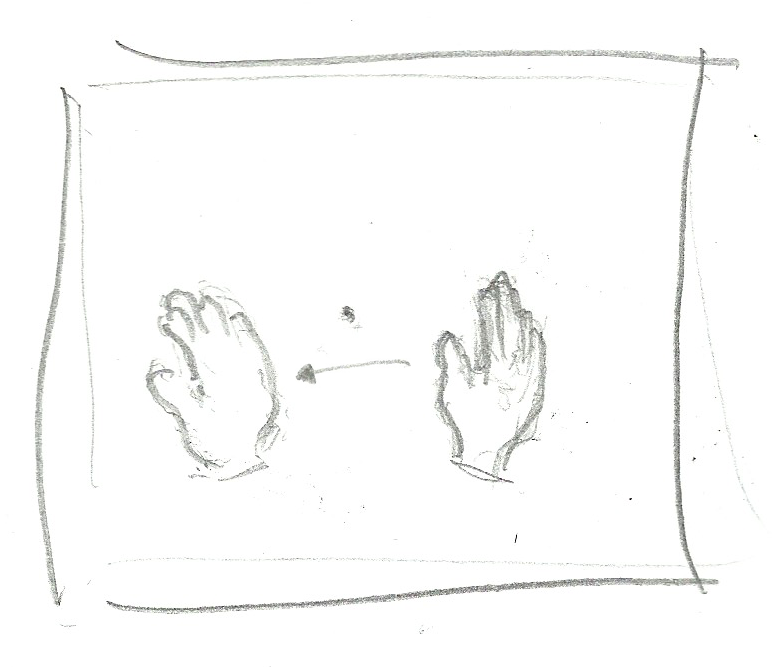
\includegraphics[width=0.35\textwidth]{fig/swipe-l-r}
  \end{center}
  \vspace{-20pt}
  \caption{Gest: brukeren sveiper hånd mot venstre}
  \label{fig:gest}
  \vspace{-7pt}
\end{wrapfigure}
Figur \ref{fig:gest} viser en typisk gest der brukeren sveiper hånda foran sensoren som befinner seg på veggen. Kanskje denne gesten betyr å skru av lyset i rommet sensoren befinner seg i. Eller kanskje gesten betyr å skru på radioen, låse opp en dør, lukke gardinene eller starte kaffemaskinen. Det er ingen begrensning på hva en enkelt gest aktiverer i form av funksjonalitet.

Når en gest utføres må enten rådataene fra sensoren eller en forståelse av dataene sendes til et system som har ansvaret for å styre hjemmet. Sensoren må være knyttet til en mikrokontroller eller tilsvarende som har ansvaret for å sende dataene videre. Dette kan enten være gjennom kabel eller trådløst. Det er mulig å programmere en mikrokontroller til å skille mellom sensordataene og forstå seks ulike gester\footnote{https://github.com/sparkfun/APDS-9960\_RGB\_and\_Gesture\_Sensor}. Dette er i seg selv bra og betyr at en enkelt sensor kan fungere som en knapp med seks forskjellige innstillinger. Hvis man også utnytter at kombinasjonen av flere gester etter hverandre kan bety egne kommandoer er styringsmulighetene mange. Det finnes et alternativ til å programmere hva de ulike dataene skal tolkes som. Alternativet er å sende rådataene til en kraftigere maskin som kan benytte maskinlæring til å forstå potensielt enda flere ulike gester.

For å utføre eksperimentet benyttet jeg først Python-scriptet \emph{process-data.py}, for å åpne tilkoblingen til den serielle porten mikrokontrolleren sender data til. Porten åpnes periodisk i noen sekunder og ber om at en gest utføres. Jeg gjennomførte 50 utførelser av hver av de 10 gestene (se figur \ref{fig:gester}), for totalt 500 treningseksempler. I illustrasjonene i figur \ref{fig:gester} indikerer en enkelt pil et rolig sveip over sensoren. Tre piler indikerer en større hastighet. Dataene fra hver gest ble lagret i individuelle filer i \emph{CSV}-format. Med dataene fra hver gest lagret i forskjellige filer, kan disse kombineres slik jeg ønsker og trene systemet til å skille mellom 2,3, eller opp til 10 gester. 

Maskinlæring handler om å la maskinen lære fra data. Dette kan enten være et forsøk på å finne ukjente sammenhenger i dataene den mates med eller det kan være å lære seg sammenhenger mellom treningseksempler og klasser. Det er dette sistnevnte scenariet jeg er interessert i. Jeg matet maskinen med data fra en gest og ga samtidig informasjon om at dataene maskinen akkurat fikk betyr "sveip til høyre". Dermed kan maskinen forsøke å danne en optimal kobling mellom dataene som kom inn da jeg sveipet til høyre og informerte om at disse dataene hørte til klassen "sveip til høyre". Med en tilstrekkelig mengde treningseksempler fra de ulike gestene skal maskinen kunne lære seg forskjellene mellom dem. Dermed vil den være i stand til å gjette riktig når en av de 10 gestene utføres senere.
\begin{figure}[h]
\begin{subfigure}{0.23\textwidth}
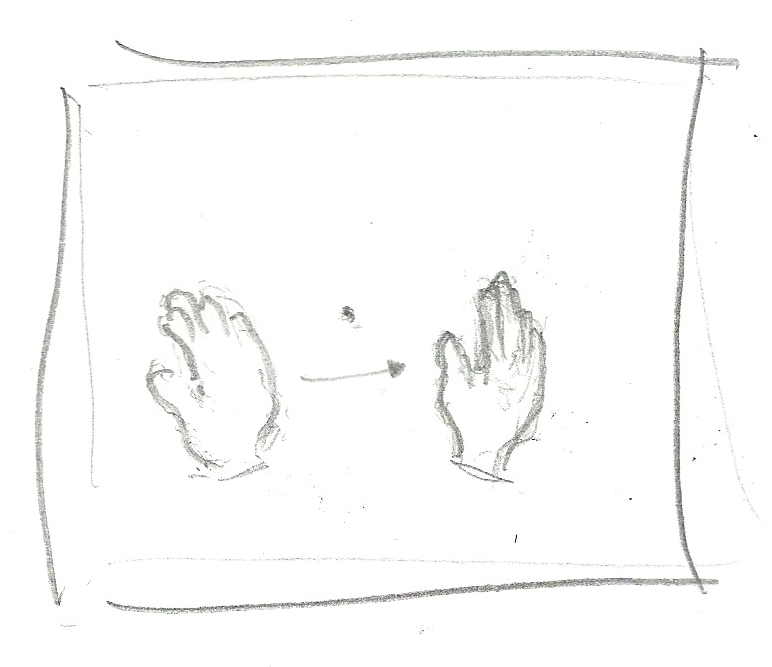
\includegraphics[width=3cm, height=3cm]{fig/swipe-r-l}
\caption{Sveip til høyre.}
\label{fig:sveip-}
\end{subfigure} 
\begin{subfigure}{0.23\textwidth}
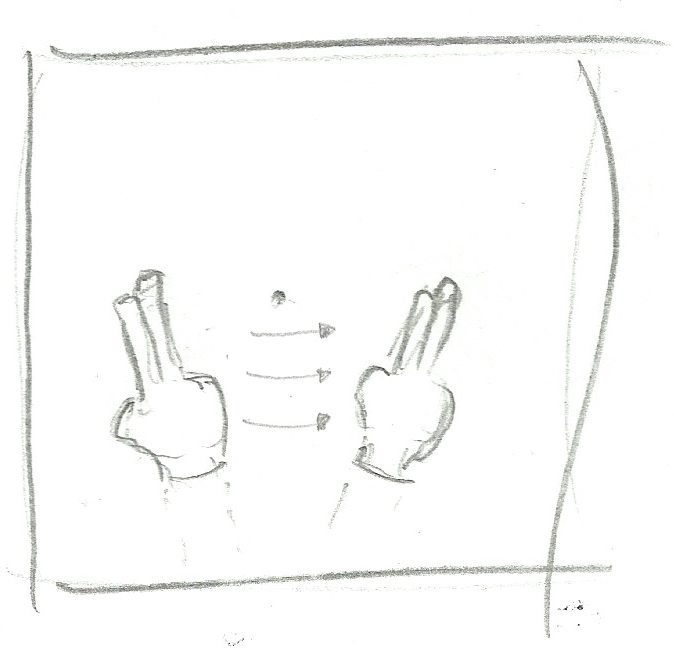
\includegraphics[width=3cm, height=3cm]{fig/flick-l-r} 
\caption{Flikk til høyre.}
\label{fig:flikk-h}
\end{subfigure}
\begin{subfigure}{0.23\textwidth}
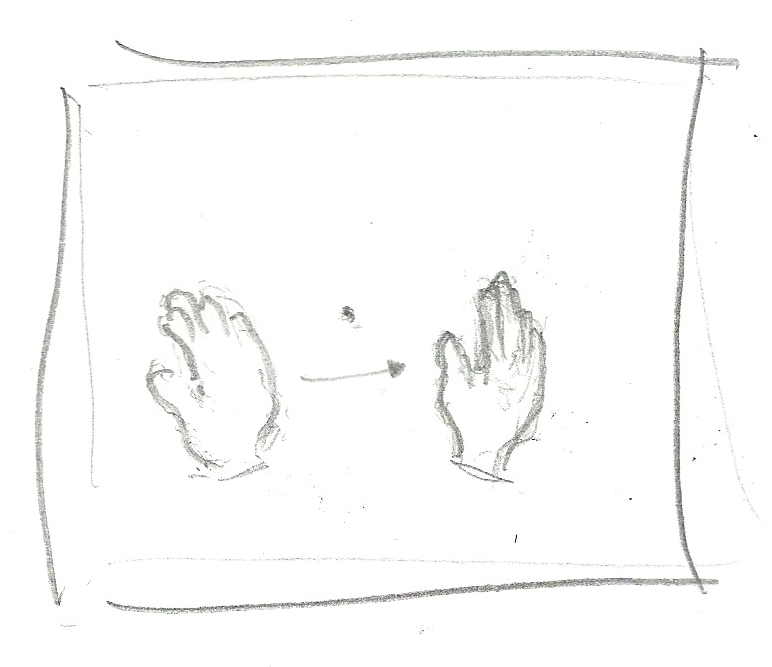
\includegraphics[width=3cm, height=3cm]{fig/swipe-r-l}
\caption{Sveip til venstre.}
\label{fig:sveip-v}
\end{subfigure} 
\begin{subfigure}{0.23\textwidth}
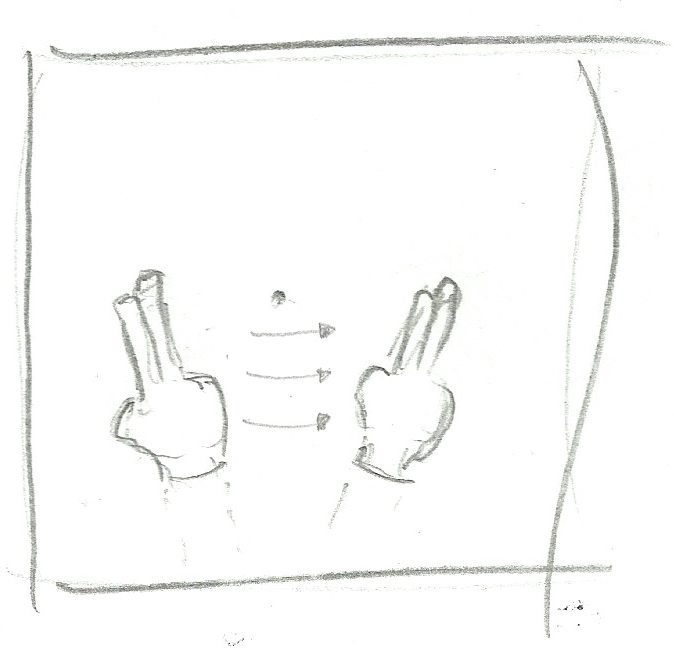
\includegraphics[width=3cm, height=3cm]{fig/flick-l-r}
\caption{Flikk til venstre.}
\label{fig:flikk-v}
\end{subfigure}
\begin{subfigure}{0.23\textwidth}
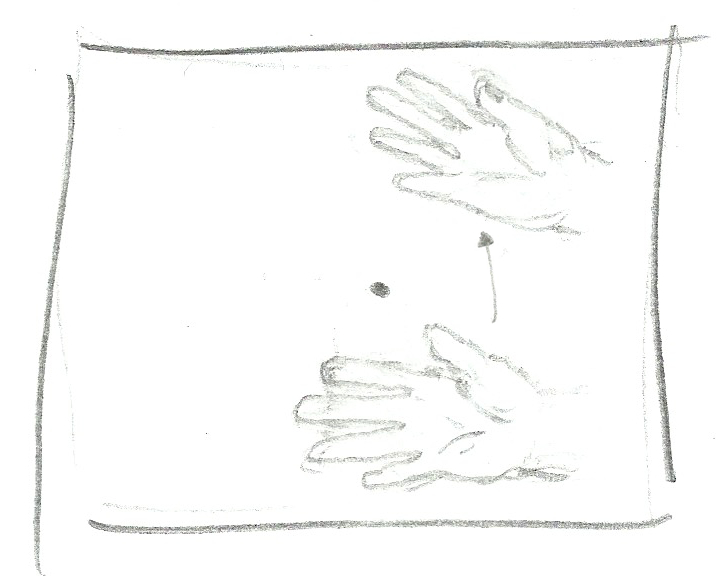
\includegraphics[width=3cm, height=3cm]{fig/swipe-d-u}
\caption{Sveip opp.}
\label{fig:sveip-opp}
\end{subfigure}
\begin{subfigure}{0.23\textwidth}
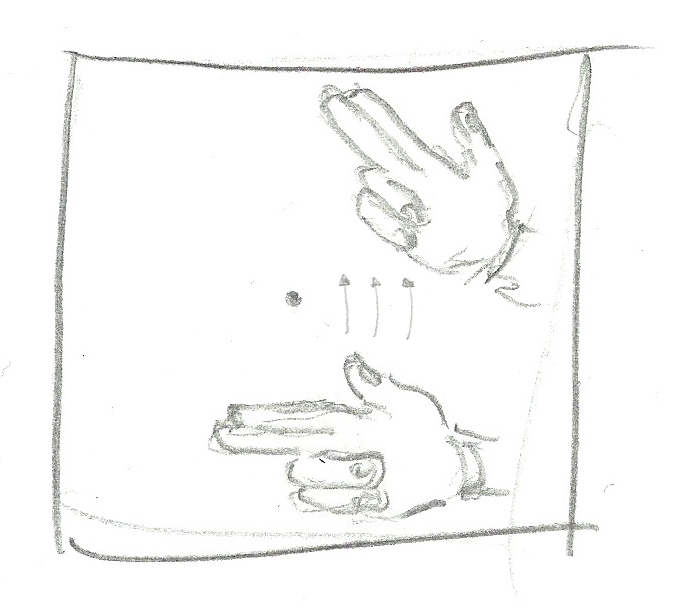
\includegraphics[width=3cm, height=3cm]{fig/flick-d-u}
\caption{Flikk opp.}
\label{fig:flikk-opp}
\end{subfigure}
\begin{subfigure}{0.23\textwidth}
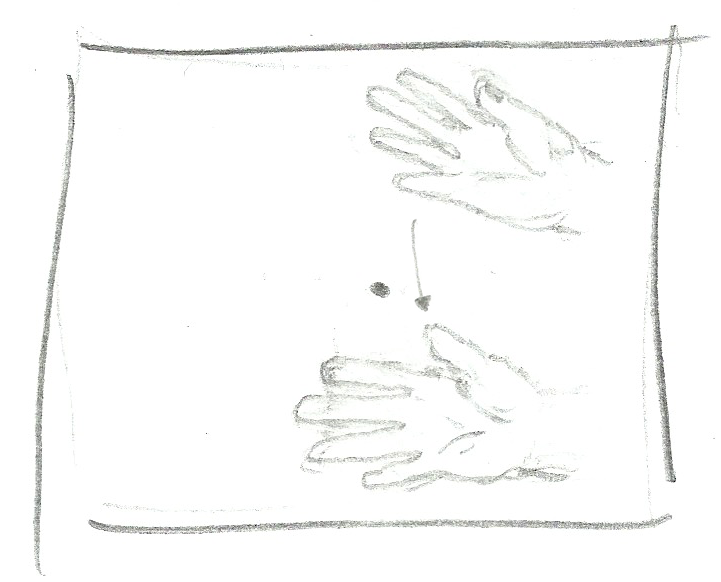
\includegraphics[width=3cm, height=3cm]{fig/swipe-u-d}
\caption{Sveip ned.}
\label{fig:sveip-ned}
\end{subfigure}
\begin{subfigure}{0.23\textwidth}
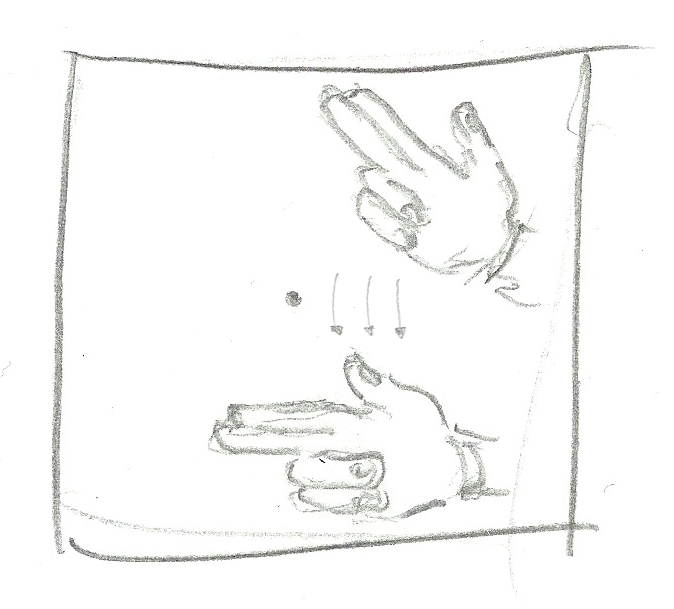
\includegraphics[width=3cm, height=3cm]{fig/flick-u-d}
\caption{Flikk ned.}
\label{fig:flikk-ned}
\end{subfigure}
\begin{subfigure}{0.25\textwidth}
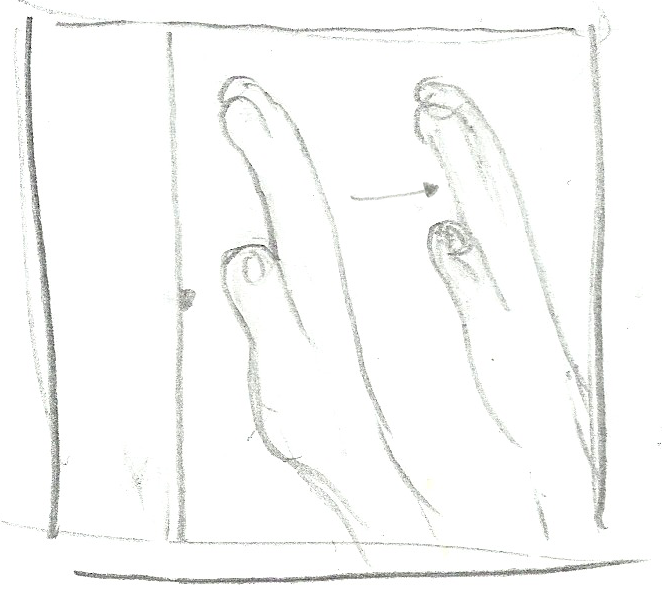
\includegraphics[width=3cm, height=3cm]{fig/near-far}
\caption{Nær - fjern.}
\label{fig:n-f}
\end{subfigure}
\begin{subfigure}{0.23\textwidth}
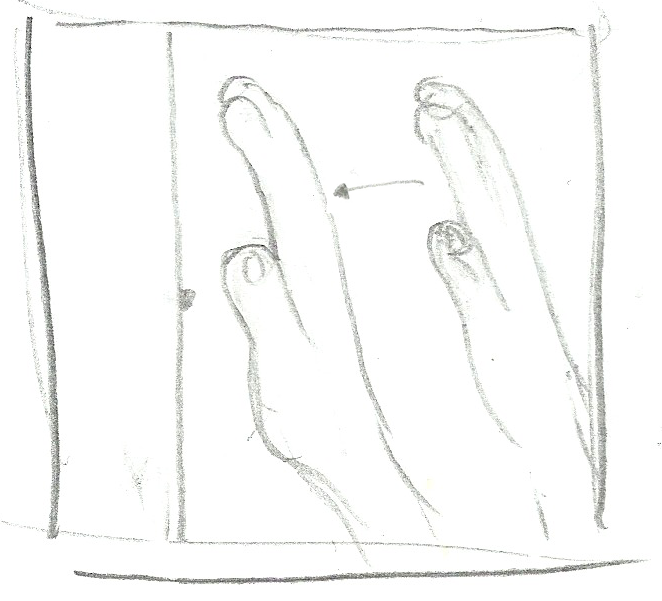
\includegraphics[width=3cm, height=3cm]{fig/far-near}
\caption{Fjern - nær.}
\label{fig:f-n}
\end{subfigure}
\caption{De 10 ulike gestene}
\label{fig:gester}
\end{figure}
Jeg benyttet Python-scriptet \emph{learning.py} for å utføre maskinlæringen. De lagrede dataene ble lastet inn og de aktuelle klassene opprettet. Jeg splittet så dataene i et treningssett og et testsett. Splittingen var 75\% til trening og 25\% til testing. Dette er et viktig steg i prosessen for å ikke overspesialisere modellen til dataene. Dersom man trener algoritmen på hele datasettet og så tester på det samme settet, er det en sjanse for at modellen blir overtilpasset. Man ønsker å finne den underliggende sammenhengen i dataene. Man ønsker ikke å danne en modell som perfekt representerer treningsdataene, men som ikke vil håndtere nye data godt. Hver modell ble trent og testet 100 ganger med et tilfeldig utgangspunkt hver gang. Sluttresultatet er et gjennomsnitt av disse 100 utførelsene, med et 95\% konfidensintervall.\\

\subsubsection*{Multimodal interaksjon gjennom tale og gester}
Mennesker i mellom kommuniserer i hovedsak med tale og det er derfor forsket mye på å få datamaskiner til å forstå og bruke denne naturlige kommunikasjonsformen. Det er liten tvil om at det er en stor drøm for mange å ha en kontinuerlig samtale med datamaskinen. I et smart hjem kunne det vært hendig å styre miljøet og enhetene, få hjelp til arbeid eller hobbyer og å gjøre oppslag etter matoppskrifter og værutsikter; alt gjennom en samtale med hjemmet.

La oss fokusere på å bruke tale til det folk bruker tale til; å gi kommandoer og å stille spørsmål. Tale har først om fremst sin plass som \emph{kommunikasjonsprogramvare}. Tale kan også ha en begrenset nytte i forbindelse med læring; som å få faktasvar på tilstanden til hjemmet, eller for å lære om været for de neste dagene. Men for å bedrive dyp og god læring kreves det en aktiv utforskning. Vi lærer best ved å peke på ting, justere dem, holde dem i hendene og ved å ha muligheten til å bevege oss rundt dem. Tale virker upassende for denne typen aktiv utforskning. Når det gjelder programvare for å \emph{skape} virker det også som om tale kommer til kort. Jeg kan forestille meg at det i framtiden blir laget verktøy der brukeren forteller datamaskinen hva som skal gjøres for å lage noe. Men arbeid som involverer en evolusjon av produktet, som kunst eller ingeniørvirksomhet, er vanskelig å beskrive med ord. Disse tingene skapes gradvis og vi manipulerer dem best med hendene våre. For meg fremstår tale hovedsaklig som en effektiv og naturlig interaksjonsform når det gjelder å gi kommandoer og å få informasjon, enten kommunikasjonen er med menneske eller maskin.

Dagens kommersielle løsninger, fra Google, Apple og andre, benytter seg av avanserte systemer for å forstå kontinuerlig tale. Med optimaliserte algoritmer og tilstrekkelig datakraft tilbyr disse aktørene talegjenkjenning med en svært høy grad av korrekthet. Men for å benytte tjenestene må taledataene som oppfattes av brukerens mikrofon, sendes til kraftige maskiner på andre siden av kloden. Der prosesseres dataene, talen forstås og resultatet returneres. Det kan være vanskelig for disse systemene å garantere en god responstid. Dersom det tar flere sekunder før et resultat returneres vil nytteverdien til talegjenkjenning raskt minke. Umiddelbar respons vil være langt mer attraktivt. Denne tilnærmingen til talegjenkjenning har også problemer rundt bevarelse av personvernet. I et hvert tilfelle hvor data forsvinner ut av brukerens kontroll kan det være problemer. Det kan tenkes at taledata til tider inneholder sensitiv informasjon, som kalenderinformasjon, søkeord, eller tilstanden til hjemmet. Dersom informasjon om hjemmets alarmsystem, tilstedeværelse av brukere eller ulåste dører forsvinner ut av hjemmet, er dette en direkte sikkerhetsrisiko. En kjeltring, ute etter gjenstander eller identiteter, kan sitte på utsiden av hjemmet og få tilgang til sensitive data om hjemmet og dets beboere.

Samsung tilbyr både tale- og gestekontroll på sine nyere Smart-TV-er. En nærmere kikk på deres \emph{global privacy policy} skapte i år oppstyr i media. Samsung tilsier seg retten til å lagre tale- og video-data for å forbedre tjenesten, samt å gi den videre til visse tredjeparter\footnote{\url{https://www.samsung.com/uk/info/privacy-SmartTV.html?CID=AFL-hq-mul-0813-11000170}}. Brukere har naturligvis vist misnøye med at alt de sier i stua kan bli tatt opp og sendt til tredjeparter. Samsung har advart brukerene om å diskutere personlig informasjon foran disse Smart-TV-ene. Personvernsbevisste brukere må altså nå passe på hva som blir sagt i sin egen stue!

Basert på diskusjonen så langt kan det se ut som talegjenkjenningsprosessen bør holdes lokal, og at man dermed unngår både treg responstid og mulig krenking av personvern. Er dette mulig i dag? Moderne telefoner, tv-er og andre enheter blir stadig kraftigere, men de er langt unna supercomputerne som for eksempel kjører Google's talegjenkjenning.

Egenskapene jeg omtalte i kapittel \ref{ch:multimodalimpl} gjør Pocketsphinx til et interessant valg som kommunikasjonsprogramvare for smarte hjem. Problemdomenet vårt tilsier at vi ønsker et system som gjenkjenner et titalls kommandoer i reelltid. Det virker derfor ikke som det er nødvendig å knytte forståelsen opp mot internettet og sende taledata ut i verden. Vi kan unngå problemene med personvern, som Samsung og andre styrer med, ved å holde alle data lokalt. Ved å benytte et begrenset vokabular ofrer vi den kontinuerlige og mer naturlig talen. Til gjengjeld får vi en garantert bevarelse av personvernet. Dette er et steg bakover i utviklingen teknologimessig, men framstår som det beste alternativet i smarte hjem.

I kapittel \ref{ch:multimodalimpl} nevnte jeg hvordan de fleste kommersielle produktene håndtere problemet med kontinuerlig lytting ved å benytte et aktiveringsord. Det finnes andre løsninger på dette problemet. Et avansert, men elegant, alternativ er å benytte stemmegjenkjenning. Her forstår systemet hvem som taler basert på talerens unike vokaltrakt. Systemet kan dermed programmeres til å kun godta kommandoer fra gjenkjente og klarerte brukere. En enklere løsning er å tilby talegjenkjenning i begrensede områder av hjemmet.
\begin{wrapfigure}{r}{0.4\textwidth}
    \vspace{-20pt}
  \begin{center}
    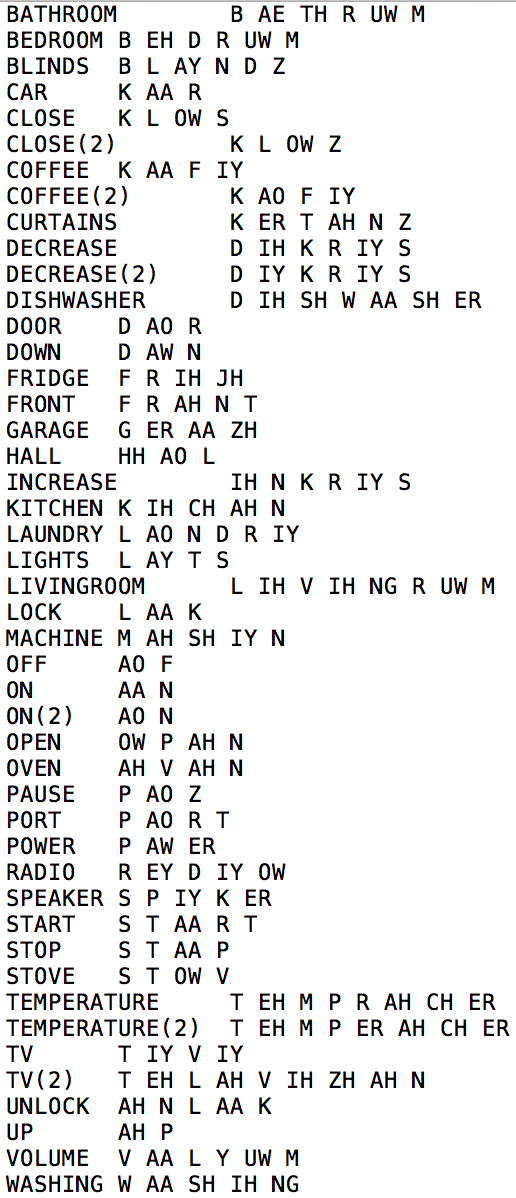
\includegraphics[width=0.35\textwidth]{fig/dictionary}
  \end{center}
  \vspace{-20pt}
  \caption{Vokabular}
  \label{fig:vokabular}
  \vspace{-7pt}
\end{wrapfigure}
For eksempel er det vanlig å tilbringe tiden alene på badet, så her kunne det vært aktuelt å la systemet lytte kontinuerlig da eventuell tale sannsynligvis vil være kommandoer til hjemmet. Jeg foreslår i dette eksperimentet å tilby kommandoutførelse gjennom tale kun dersom det også følger med en gest. Dette betyr at brukeren må stå foran enheten for å styre hjemmet. Enten kan en gest aktivere lyttingen, eller hjemmet kan lytte kontinuerlig, men kommandoer blir kun aktivert dersom en gest også utføres.

Pocketsphinx trenger et vokabular slik at den kan knytte taledata til ord og setninger. Man skriver en liste med setninger eller enkeltord man ønsker at systemet skal forstå. Deretter kan man benytte et språkmodell-verktøy til å få laget en språkmodell og et vokabular. Jeg laget en ordliste med 38 elementer. Jeg valgte først å ta med substantiver; steder og ting i hjemmet, som "kitchen", "bedroom", "dishwasher" og "radio". Det er også andre substantiver som beskriver ting eller egenskaper ved mange av rommene eller apparatene: "lights", "temperature", "blinds", "curtains", "volume" og "power". Til sist er det med verb og preposisjoner, som "on", "up", "start", "increase" og "lock". Med et slikt vokabular kan brukeren potensielt styre det smarte hjemmet med en stor grad av kontroll.

Figur \ref{fig:vokabular} viser det resulterende vokabularet etter at verktøyet har prosessert en liste med ord. Vi ser at verktøyet har forstått ordene som engelsk og har tilført data om engelsk uttale til listen. I noen tilfeller, som for "TV", er det flere alternative uttalser. Jeg skrev inn "TV" i ordlisten, og verktøyet har laget en forståelse for både "TV" og "television".

Jeg har allerede pekt på problemene med å kontinuerlig lytte etter tale. Dersom systemet er slik at tale og gester må kombineres for effekt, kan tale benyttes for å peke ut substantivet, eller hva som skal opereres, og gester kan brukes for å utøve verbet eller preposisjonen. For eksempel kan brukeren si "kitchen lights" og samtidig utføre et sveip mot høyre, for å skru på kjøkkenlyset. Eller brukeren kan heve persiennene ved å si "blinds" og sveipe hånda oppover. Figur \ref{fig:multimodalvisualisert} er en illustrasjon der input fra både gester og tale tegnes til det samme lerretet med noe forskjellige skriftstørrelse og farger.
\begin{figure}
\centering
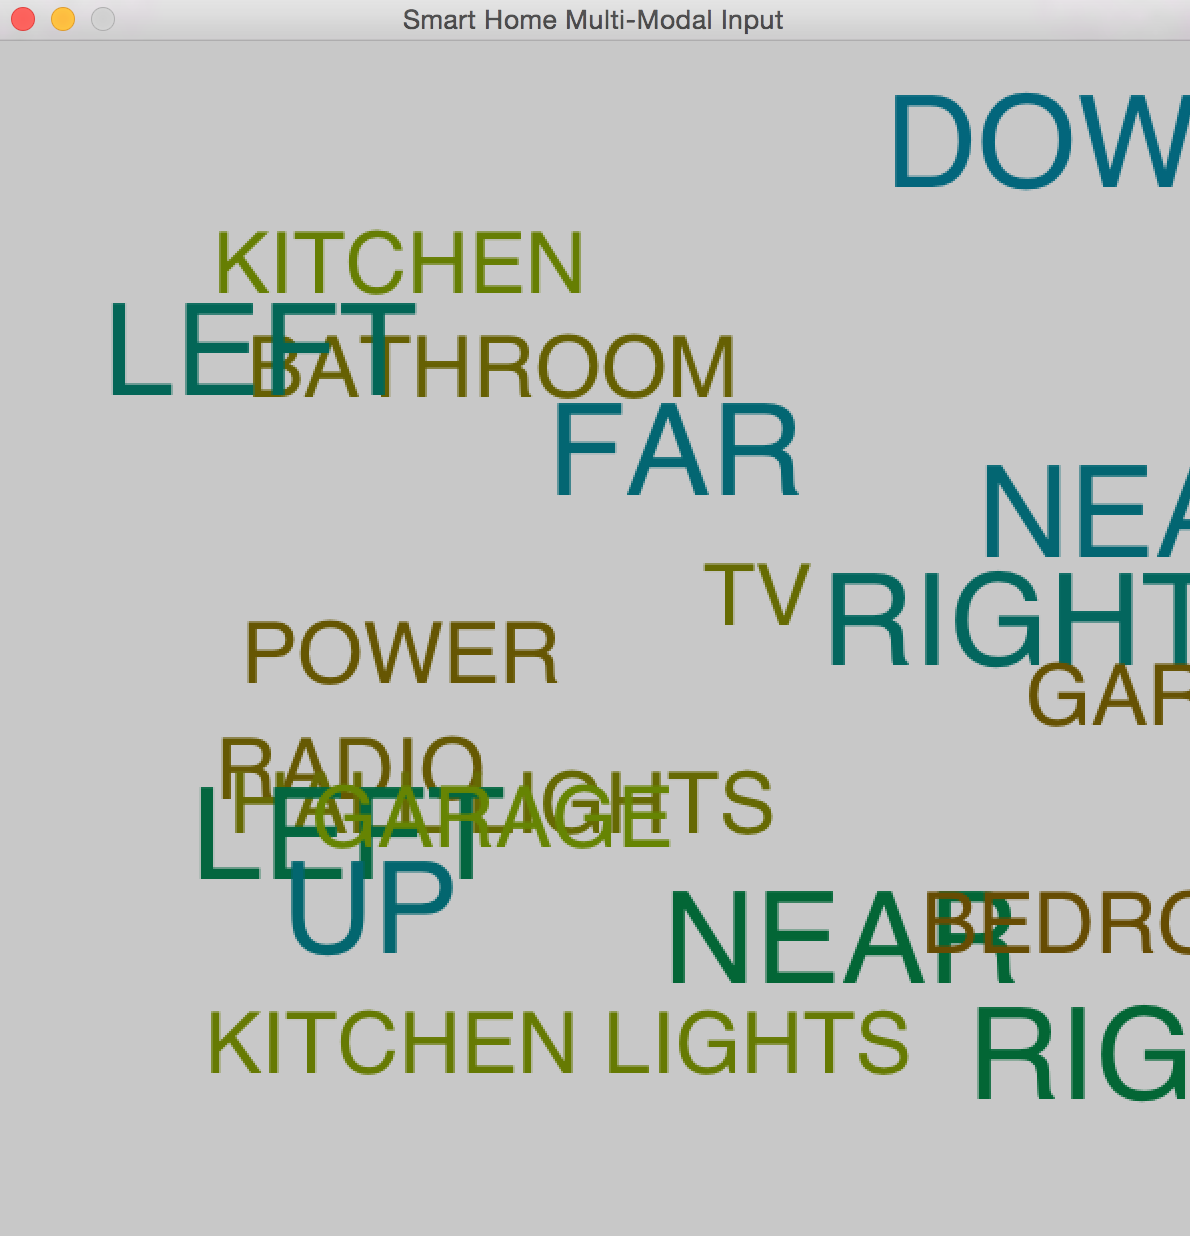
\includegraphics[scale=0.2]{fig/screenshot_project2}
\caption{Multimodal input visualisert}
\label{fig:multimodalvisualisert}
\end{figure}
Denne enkle grafikken demonstrerer at dataene fra begge inputkilder er likestilt og at ingen data går tapt, selv med input fra flere simultane kilder. Dette er en form for \emph{late/decision-level fusion}, der de to inputkildene forstås hver for seg og resultatene kombineres og vises grafisk.\\

\subsubsection*{Kombinasjoner}
I det tredje eksperimentet definerte jeg 42 abstrakte gester, skapte data fra disse gestene og benyttet maskinlæring for å skille mellom dem.\begin{figure}
\centering
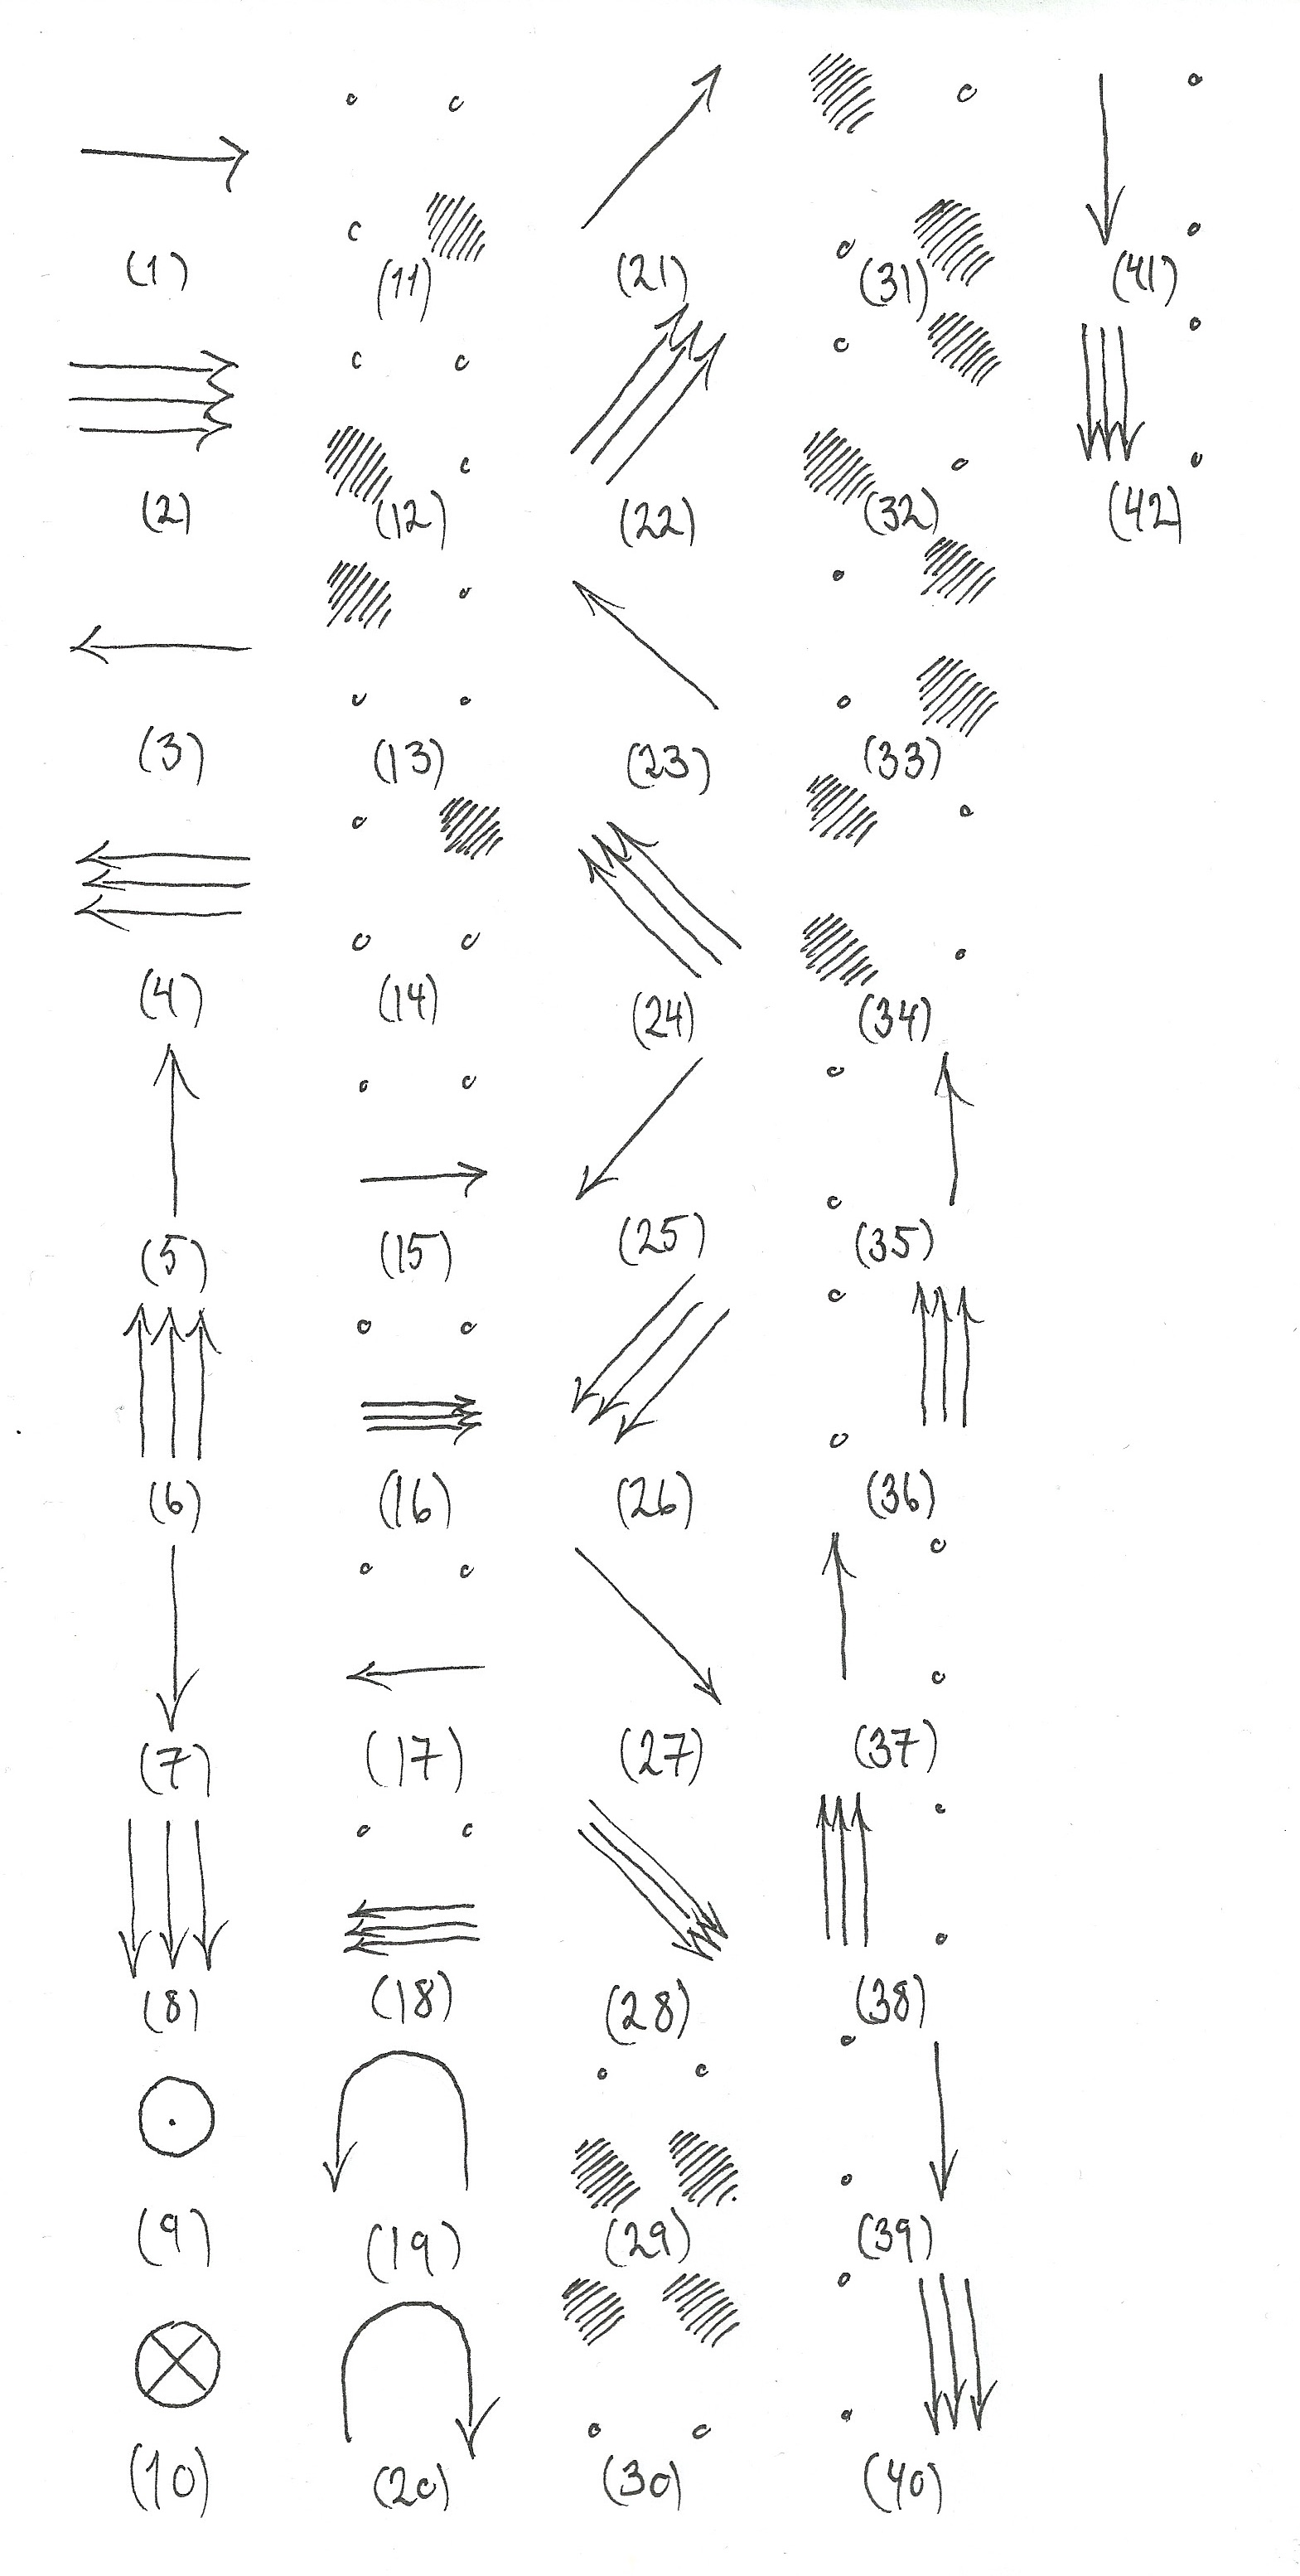
\includegraphics[scale=0.2]{fig/42-gestures}
\caption{42 gester}
\label{fig:42}
\end{figure}Deretter ble andre data fra sensorene forsøkt utnyttet for å skape en verdifull applikasjon i hjemmet. Et stort vokabular av abstrakte gester er i praksis et tegnspråk. Derfor burde alle retningslinjer for tale også gjelde i dette tilfellet. Teknologien fungerer best som kommunikasjonsprogramvare og jeg spår begrensninger innen de to andre kategoriene.

Figur \ref{fig:42} er en illustrasjon av de 42 gestene. De 10 første er de samme som i eksperiment 1. En pil indikerer et sveip i pilens retning med normal hastighet. Tre piler indikerer en høyere hastighet. Gestene 9 og 10 er gester der hånda starter enten nære eller fjernt fra sensoren, og føres i den motsatte retningen. De nye gestene er gester som nr 11; her er de fire sensorene tegnet opp, og en av dem er tildekt av en hånd. Jeg utførte denne delen av eksperimentet på samme vis som eksperiment 1. Dataene ble først produsert for hånd og deretter ble modeller trent med maskinlæring. Da det her var snakk om 42 ulike gester tok jeg meg bare tid til å lagre 10 treningseksempler av hver gest.

Den andre delen av hypotesen innebar å utforske de andre egenskapene sensoren har.\begin{figure}[h]
\centering
\begin{subfigure}{0.19\textwidth}
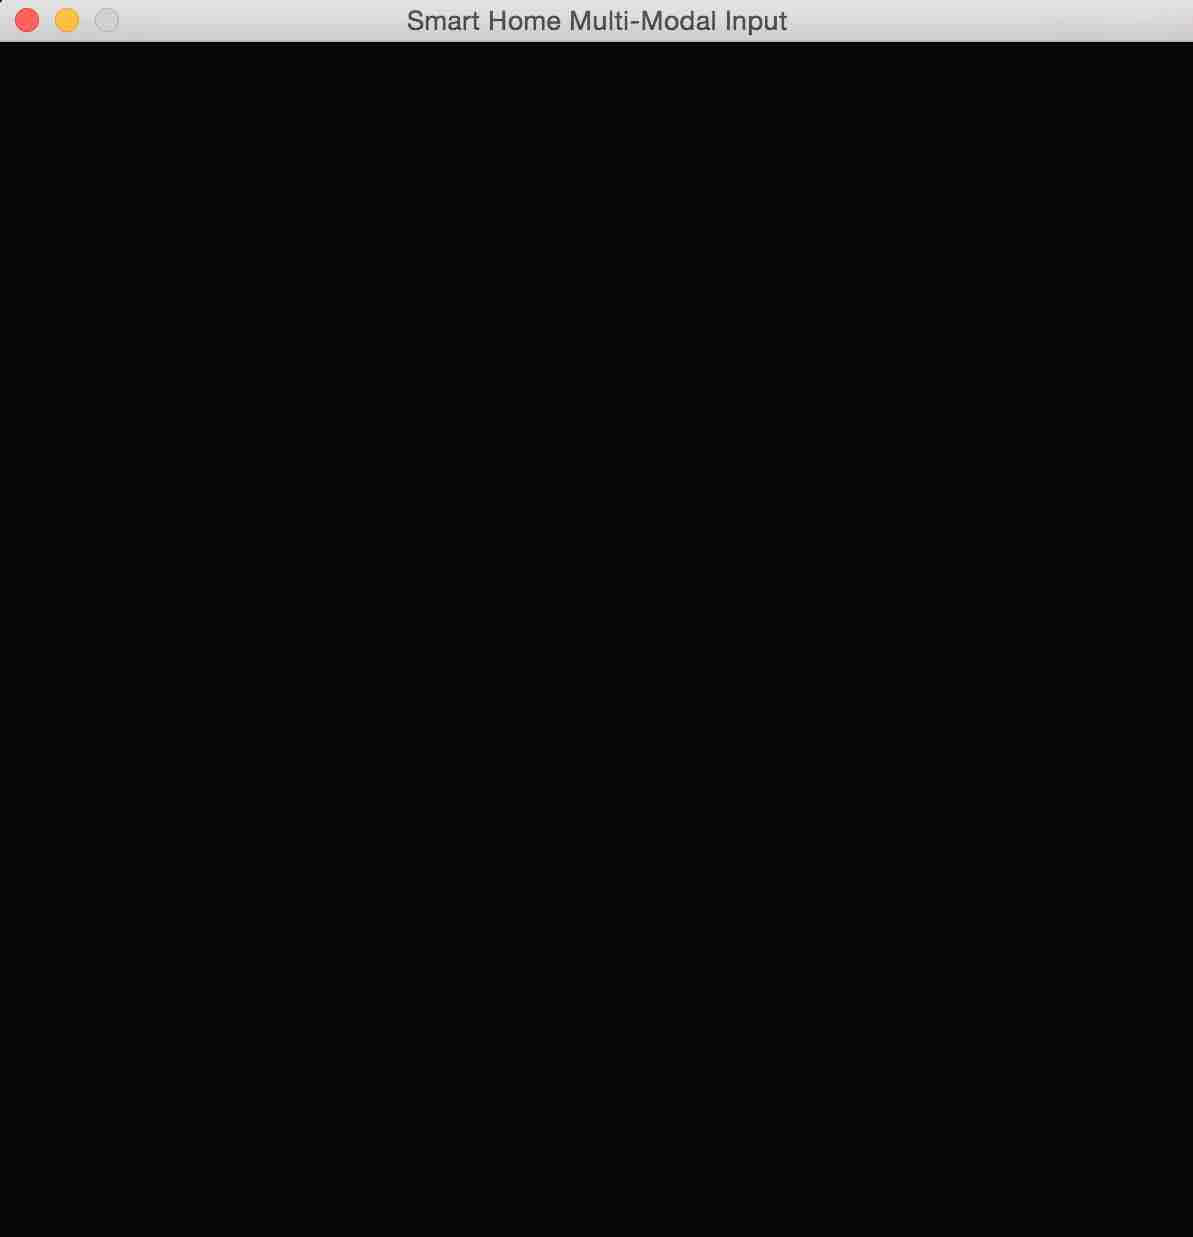
\includegraphics[width=3cm, height=3cm]{fig/light-1}
\caption{}
\label{fig:light-1}
\end{subfigure}
\begin{subfigure}{0.19\textwidth}
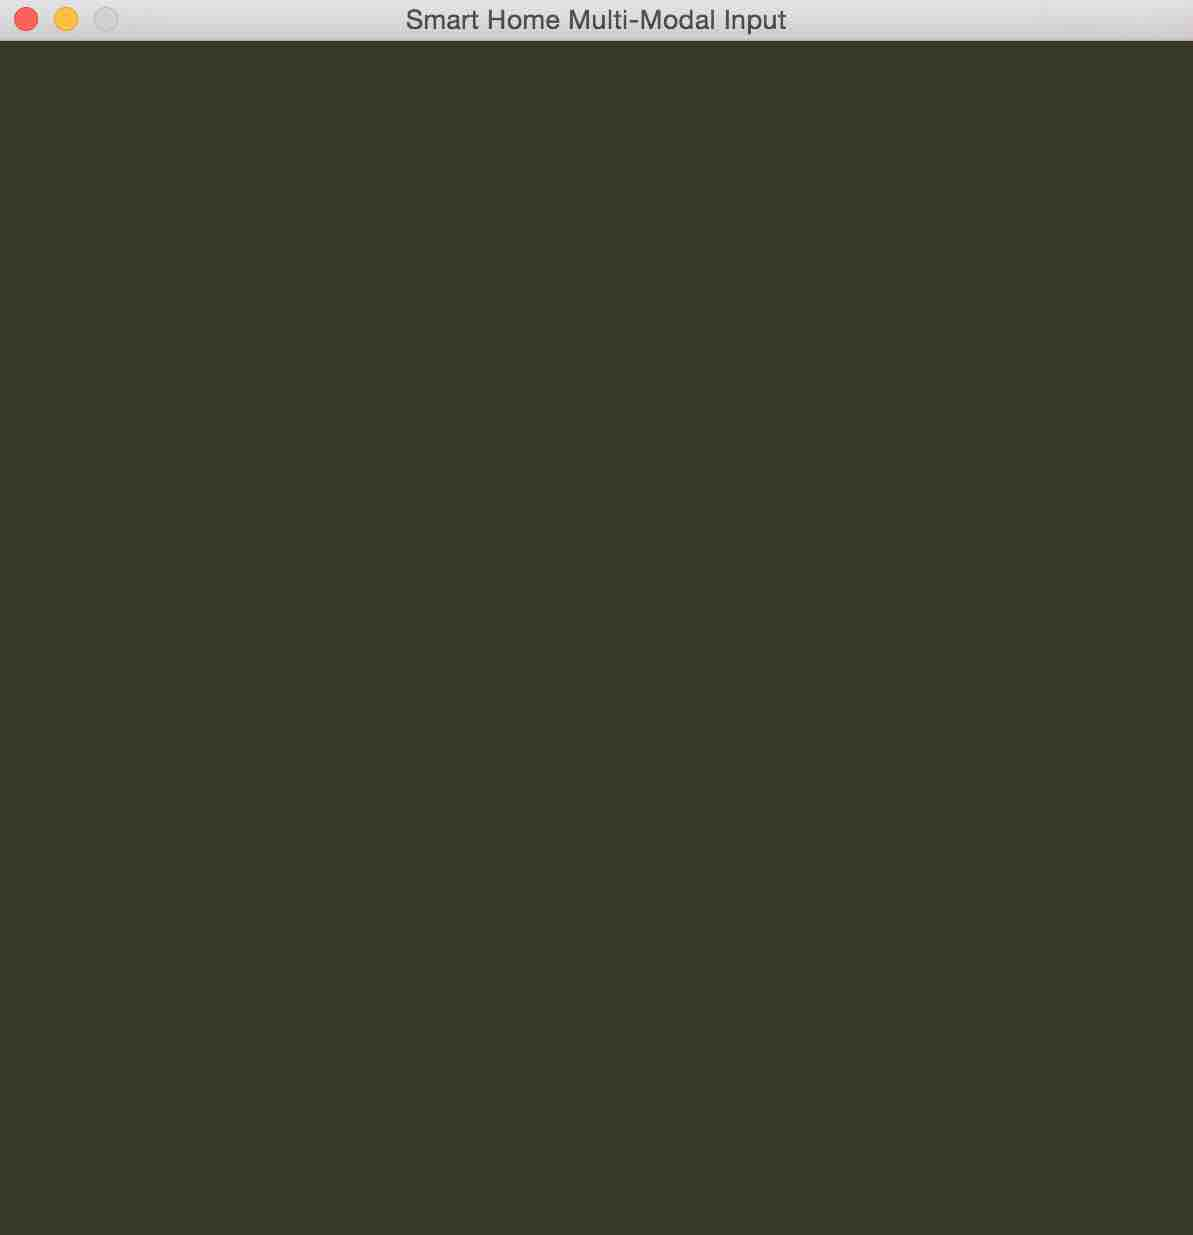
\includegraphics[width=3cm, height=3cm]{fig/light-2}
\caption{}
\label{fig:light-2}
\end{subfigure}
\begin{subfigure}{0.19\textwidth}
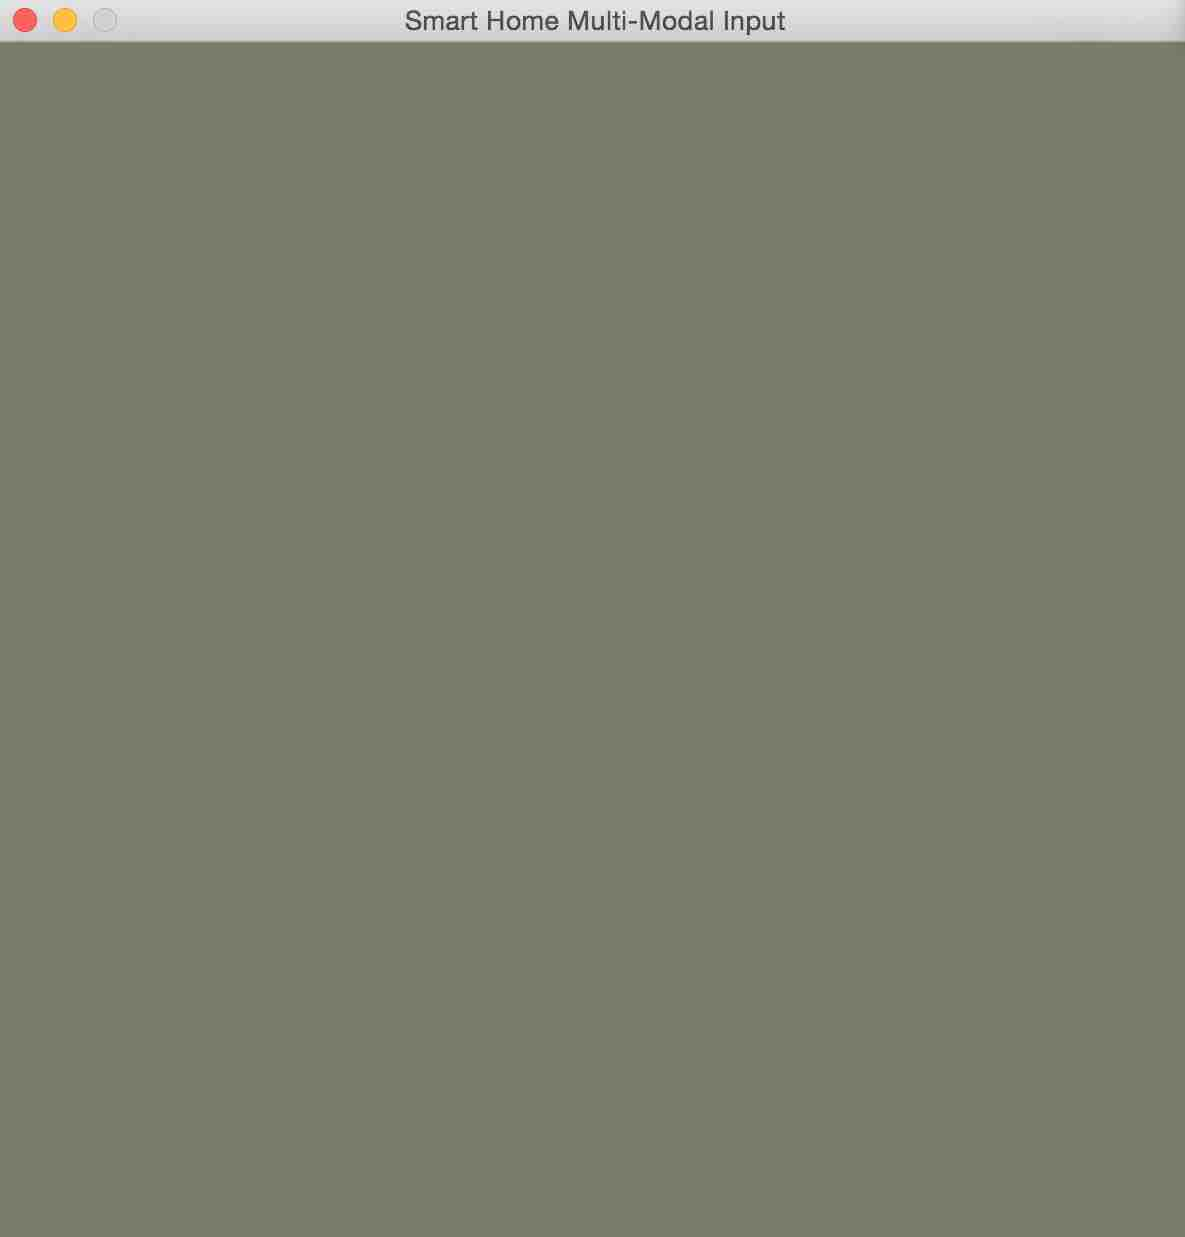
\includegraphics[width=3cm, height=3cm]{fig/light-3}
\caption{}
\label{fig:light-3}
\end{subfigure}
\begin{subfigure}{0.19\textwidth}
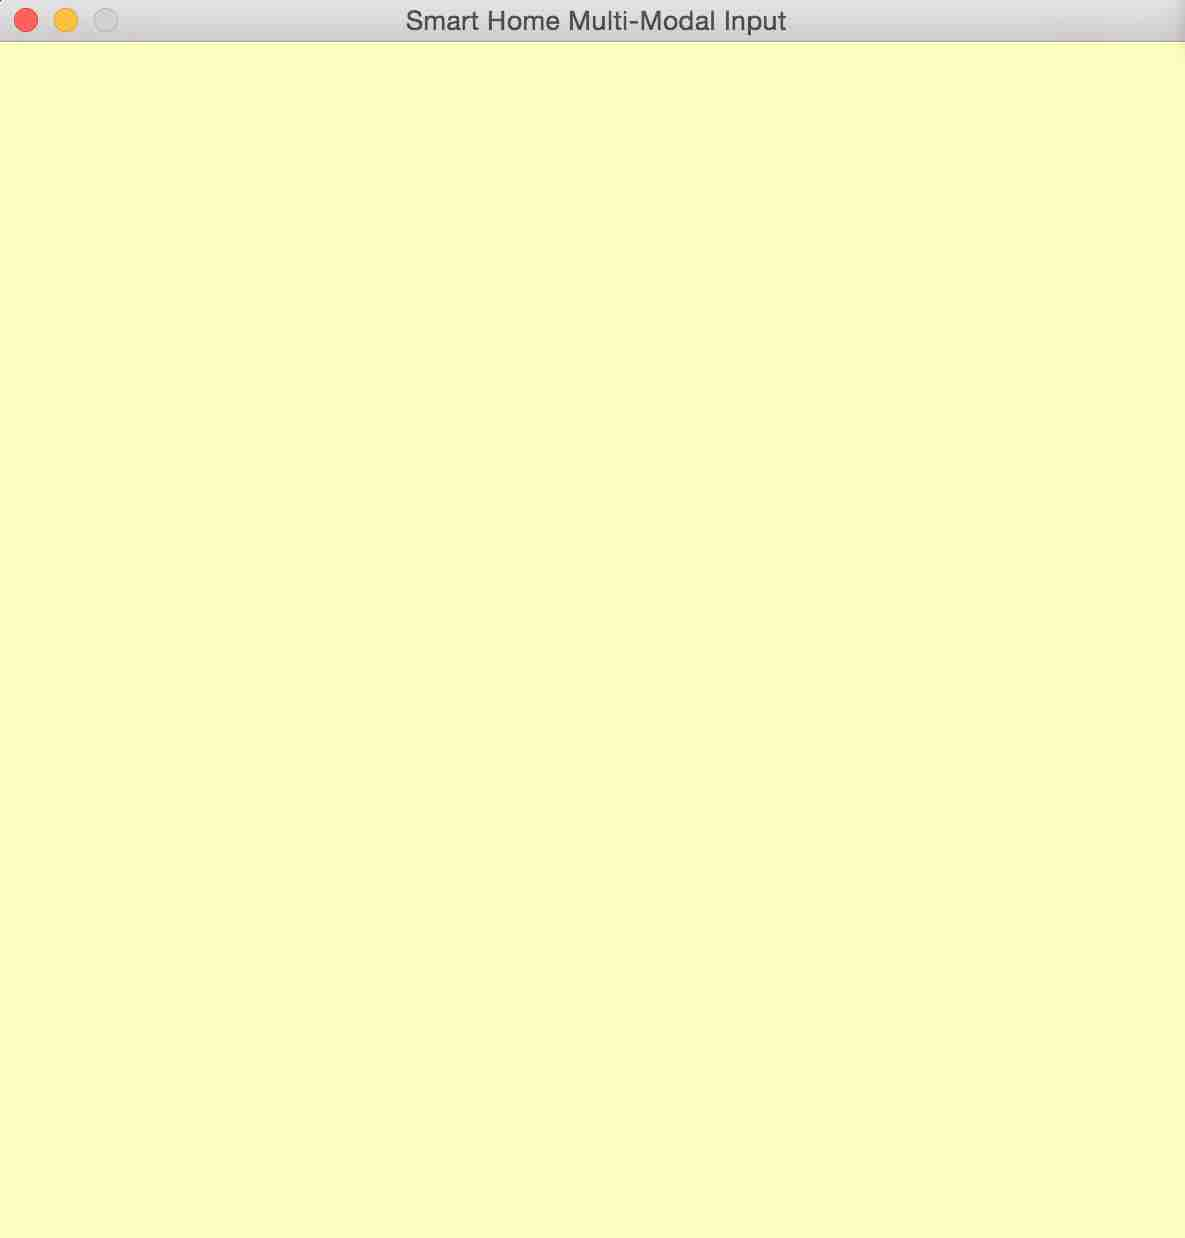
\includegraphics[width=3cm, height=3cm]{fig/light-4}
\caption{}
\label{fig:light-4}
\end{subfigure}
\begin{subfigure}{0.19\textwidth}
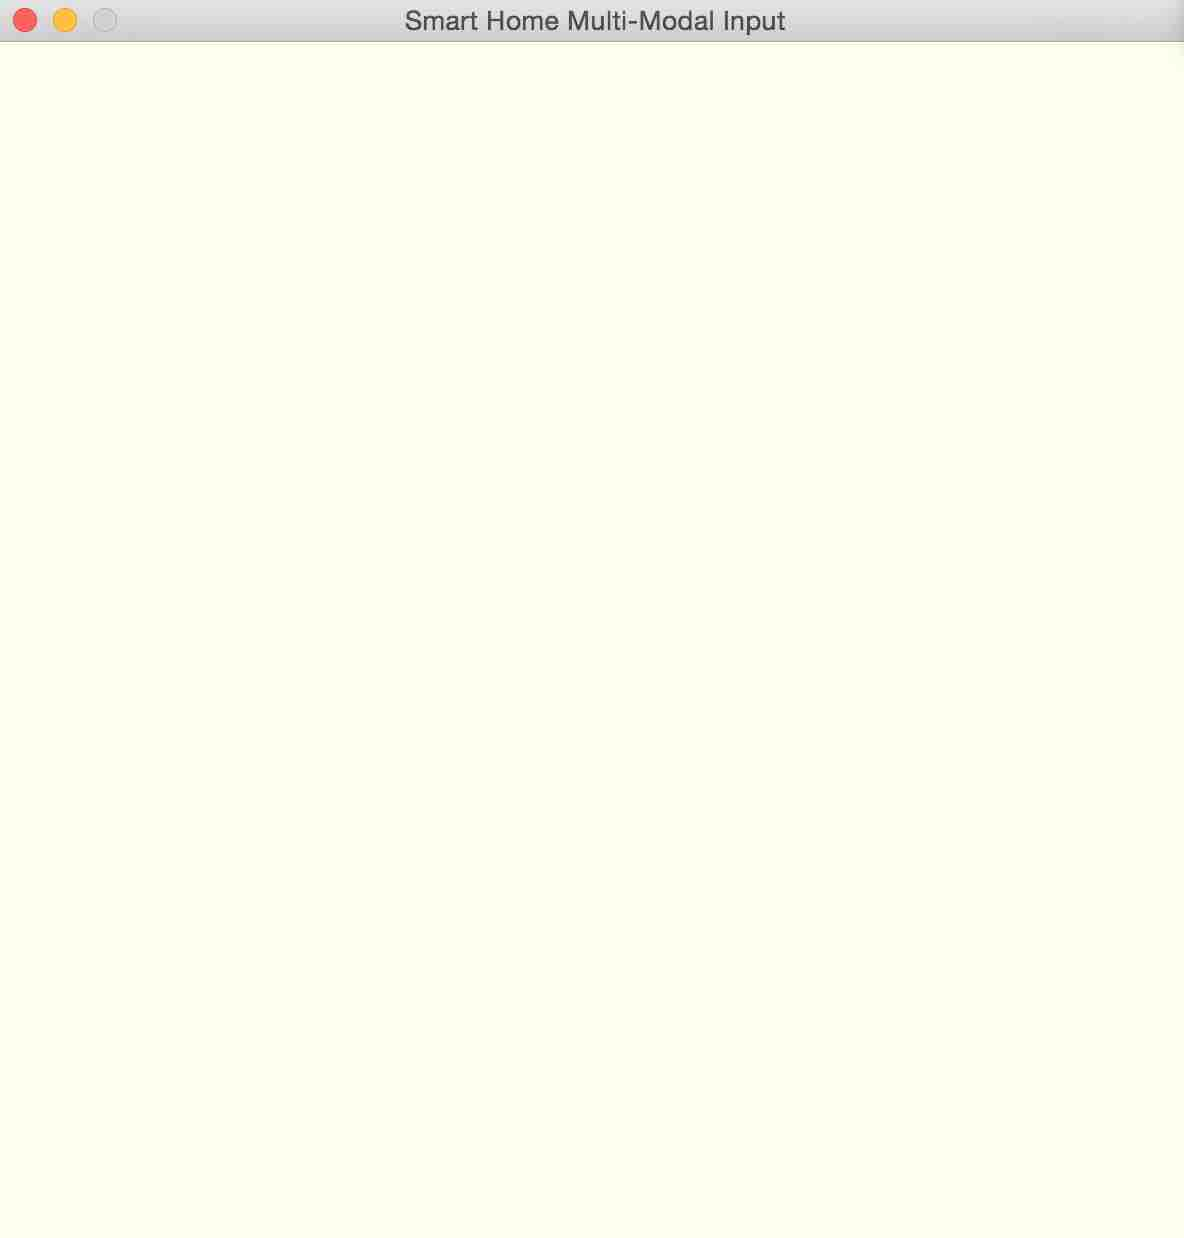
\includegraphics[width=3cm, height=3cm]{fig/light-5}
\caption{}
\label{fig:light-5}
\end{subfigure}
\caption{Dimmeeffekt}
\label{fig:light}
\end{figure}Jeg kom opp med følgende: benytt nærhetssensoren som en reguleringsmekanisme for ikke-binære innstillinger. Figur \ref{fig:light} viser denne interessante bruken av nærhetssensoren, kombinert med tale. Nærhetssensoren gir data om hvor nære et objekt befinner seg. Brukeren kan uttale hvilket apparat hun ønsker å styre og deretter dynamisk styre innstillingsnivået ved å variere avstanden mellom hånda og sensoren. Eksempelbruk kan være å regulere volumet fra høytalere, temperatur eller lysstyrke, som illustrert i figur \ref{fig:light}.\\

\subsubsection*{Kontekstdrevet brukergrensesnitt}
Som regel når en person bruker programvare er det ikke for å skape noe, men for å lese, observere, utforske og lære. Folk er ute etter å ordne egne tanker. Datamaskinen er et medium for å spørre spørsmål, gjøre sammenligninger og dra konklusjoner. Det aller meste av programvare er altså \emph{informasjonsprogramvare}. 

Informasjonsprogramvare er et medium for visuell kommunikasjon. Utseende og hvordan informasjon presenteres bør være i fokus. Hva er den relevante informasjonen? Hva vil brukeren vite? Hvordan kan data vises på den mest effektiv måten? Kan teknikker fra grafisk design anvendes for å lede brukerens blikk mot løsningen?

Delen av grafisk design mest relevant til programvare er det \citet{tufte01} kaller informasjonsdesign; bruken av bilder for å uttrykke informasjon av interesse for brukeren. En god grafisk designer posisjonerer informasjonen slik at leseren kan få svar på spørsmål, gjøre sammenligninger og trekke slutninger. Når programvareutvikleren definerer en visuell representasjon i programmet sitt, utføres en form for grafisk design, nettopp fordi det handler om å definere og posisjonere bildene brukeren skal forstå.
\begin{figure}
\centering
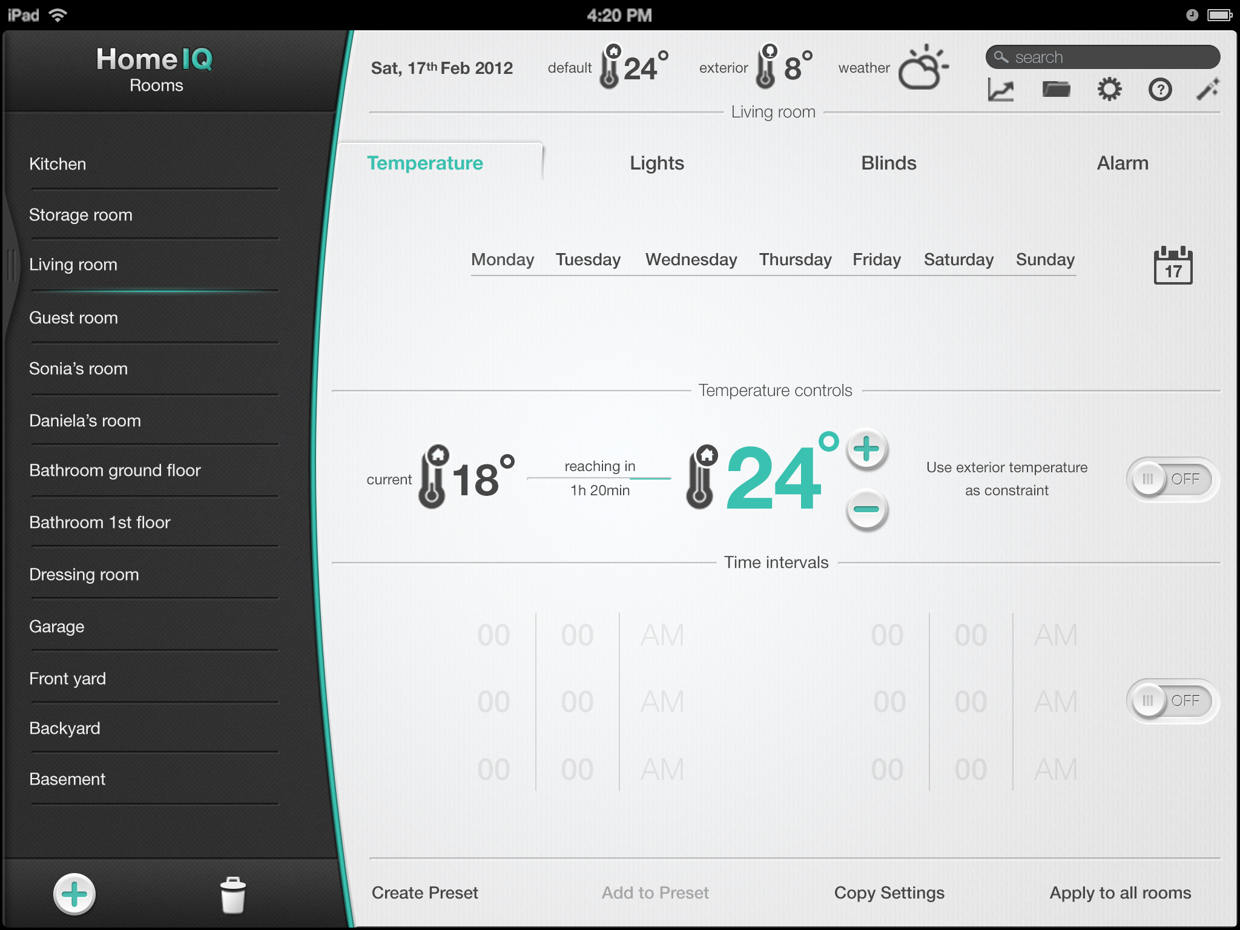
\includegraphics[scale=1.25]{fig/typical_ui_homeiq}
\caption{Brukergrensesnitt med fokus på interaksjon}
\label{fig:homeiq}
\end{figure}
Figur \ref{fig:homeiq} viser et brukergrensesnitt jeg fant på en nettside der folk viser fram prosjekter innen interaksjonsdesign\footnote{Design av Calin Giubega \url{http://www.studentshow.com/gallery/HomeIQ-Smart-Home-System/7740705}, gjenbrukt under creative commons-lisens \url{https://creativecommons.org/licenses/by-nc-nd/3.0/}}. Jeg har sett flere brukergrensesnitt for smarte hjem og dette er det beste jeg har funnet. Grensesnittet er pent å se på og det ser ut til å tilby mange innstillinger. Men hvorfor må brukeren trykke på alle knappene for å lære om hjemmet? Dataene fra et smart hjem er svært rike, med sensorer, apparater og aktuatorer. Hvorfor viser vi ikke mer av den tilgjengelige informasjonen?

Her er noen spørsmål brukeren kan ha til det smarte hjemmet:
\begin{itemize}
\item Hvor lenge er det til vaskeprogrammet er ferdig?
\item Står lyset på i garasjen?
\item Hva er temperaturen i stua nå?
\item Trenger jeg å handle inn matvarer?
\item Er ytterdøra og garasjeporten låst for natta?
\item Står det på unødvendig lys og varme i rom vi sjeldent bruker?
\item Hvor mye strøm brukte vi forrige måned?
\end{itemize}
Hvordan kan disse spørsmålene best besvares? I grensesnittet i figur \ref{fig:homeiq} må brukeren ha en interaksjon med systemet; han må lete seg gjennom estetiske menyer for å finne informasjonen. \citet{tufte01} har regler for grafisk design og den første er "framfor alt, vis dataene". Vi bør designe mot å kunne svare på spørsmål ved å vise dataene. En godt designet informasjonsgrafikk kan nærmest nøde brukeren til å stille og svare spørsmål, gjøre sammenligninger og dra slutninger. Dette oppnås ved å utnytte øyets egenskaper til å håndtere store mengder visuell data og gjenkjenne mønstre og sammenhenger. Dette henger sammen med Schneidermans argument i \ref{directmanipulation}. Men i stedet for å tilby alle mulige knapper, kan vi i stedet bare vise dataene!

Tilsvarende viktig som hva slags data som vises, er hvor dataene vises. Grafikkelementer kan plasseres på bestemte steder for å utnytte vår romforståelse. Desverre er eksisterende programvare for smarte hjem presentert for å maksimere estetikk, ikke for å framheve sammenhenger i dataene. Grensesnittet i figur \ref{fig:homeiq} er pent å se på, men setter behagelig interaksjon foran presentasjon av dataene. Vi kjenner hjemmene våre som fysiske steder. Vegger, dører, møbler og apparater har geografiske posisjoner i forhold til hverandre. Mennesket fant for mange å siden en effektiv abstraksjon for å representere geografisk data, ved \emph{kartet}. Å vise informasjon om hjemmet som et kart utnytter vår eksisterende kunnskap om de romlige relasjonene i hjemmet.
\begin{figure}
\centering
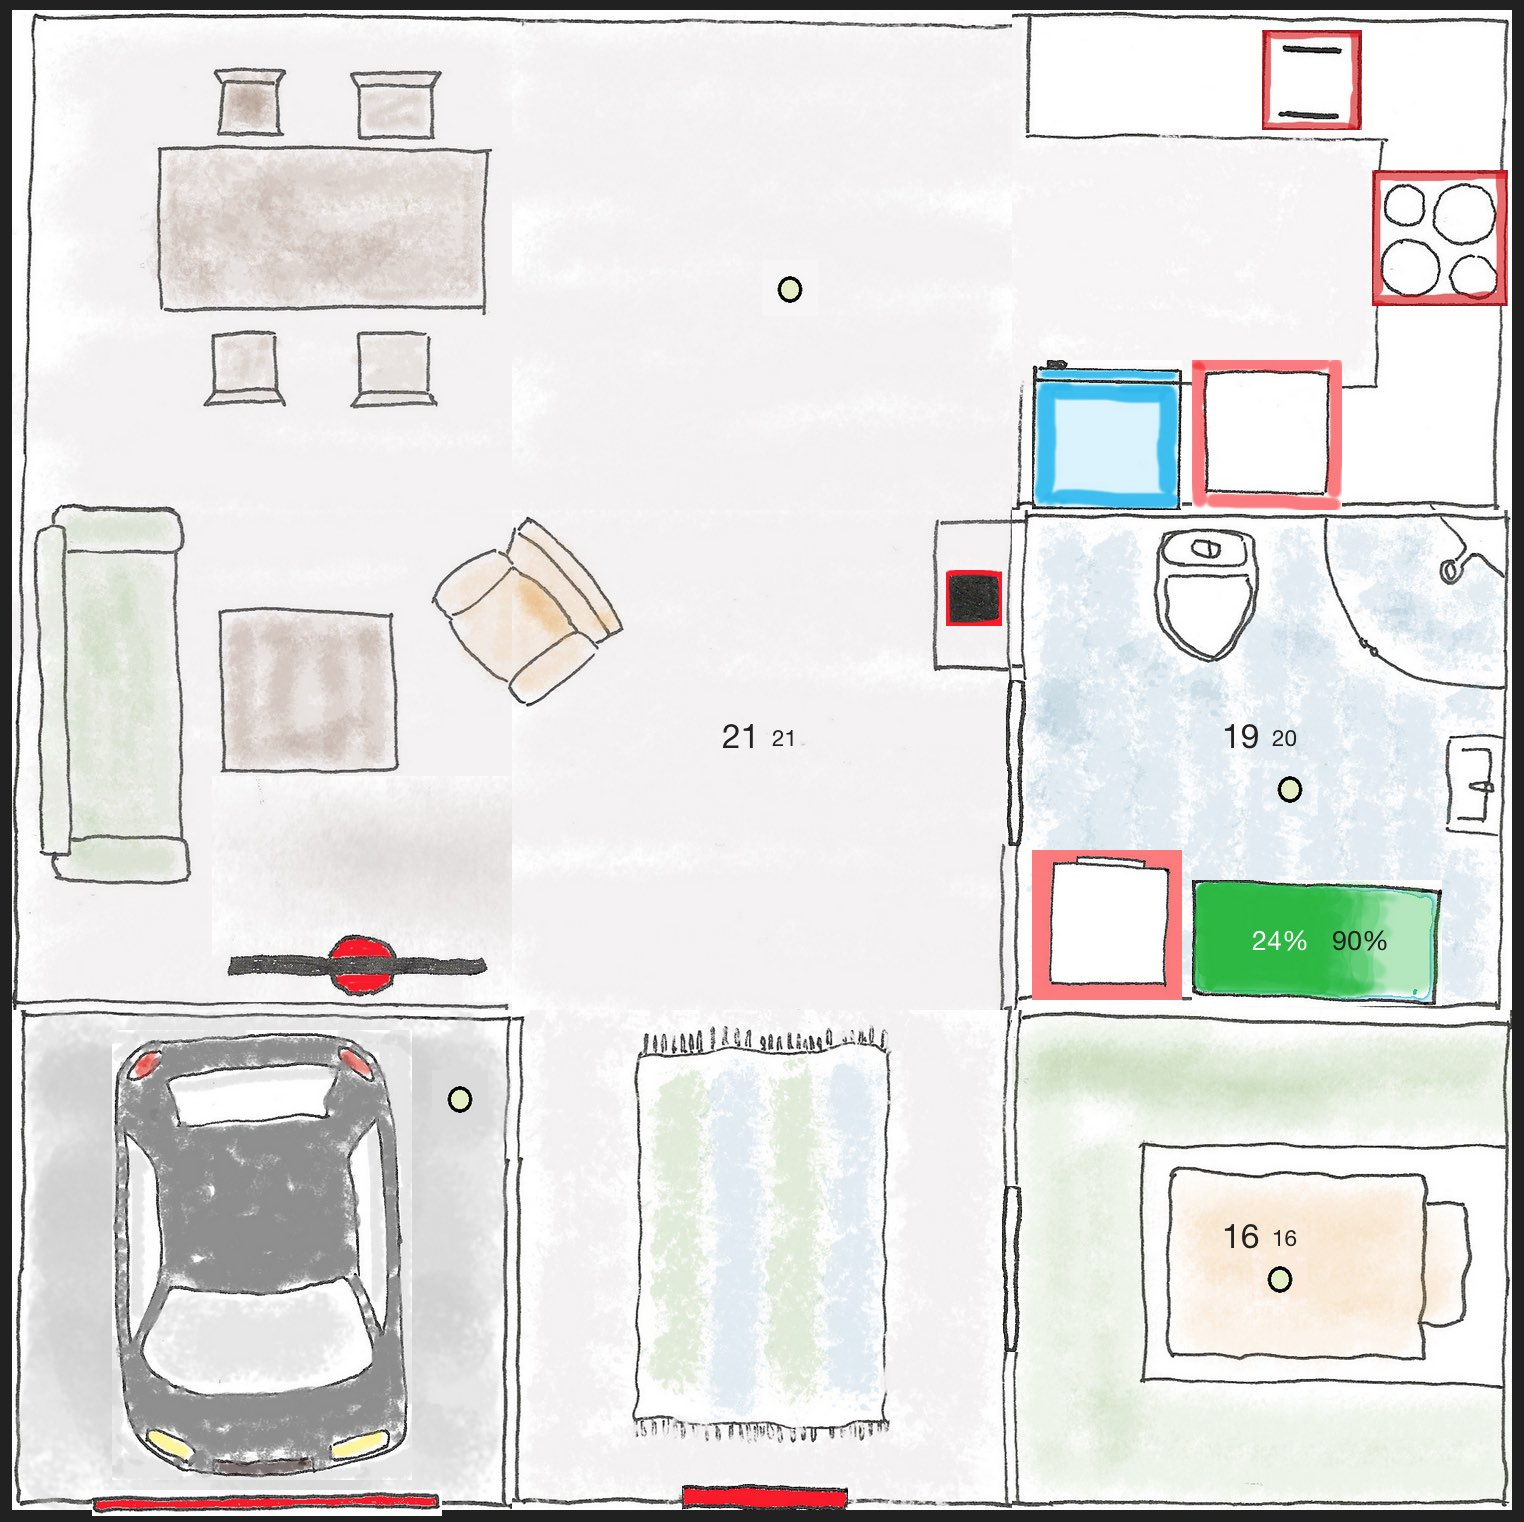
\includegraphics[scale=0.28]{fig/smarthome}
\caption{Smart hjem som grafisk design}
\label{fig:smarthjemgrafisk}
\end{figure}
Figur \ref{fig:smarthjemgrafisk} presenterer hjemmet som et to-dimensjonalt kart\footnote{Programvaren kan testes på \url{https://thesmarthome.herokuapp.com/}}. Hva slags funksjonalitet skal dette grensesnittet ha? Hva er en rimelig reaksjon fra denne type programvare, når brukeren trykker på ulike apparater? Å klikke på en lysbryter (små, blekt gule sirkler) bør naturligvis skru av eller på lyset. Å klikke på kjøleskapet eller vaskemaskinen bør enten skru av og på eller gi mer informasjon om disse apparatene. Dersom en bruker trykker på en knapp og ingenting skjer, er det vanskelig å forstå om handlingen utførte noe som helst. Brukeren får ikke muligheten til å evaluere en respons og la den lede til en ny handling. Interaksjon med brukergrensesnittet skaper kontekst. Enhver interaksjon bør gi en merkbar forandring i grafikken. Å gi direkte tilbakemelding reduserer mengden manipulasjon brukeren må utføre for å nå en tilstand der den ønskede informasjonen er tilgjengelig. I stedet for å vite navnet på en gjenstand eller et rom kan brukeren peke på kartet og si "der!". Dette vil være svært viktig i en situasjon i framtiden der hjemmet har et stort antall apparater som er koblet til nettet. \emph{Feedback-loopen} med denne løsningen er svært tett; dersom brukeren pekte på et element som kan interageres med, oppdateres grensesnittet umiddelbart. Brukeren ser alltid informasjonen om hjemmet. Dersom det som vises ikke er konfigurasjonen brukeren ønsker, kan det forandres på stedet. Det er ingen \emph{OK}, \emph{submit} eller \emph{apply}-knapp. Kartet viser alltid den nåværende tilstanden til hjemmet.\\
\begin{figure}[ht]
\centering
\begin{subfigure}{0.32\textwidth}
\centering
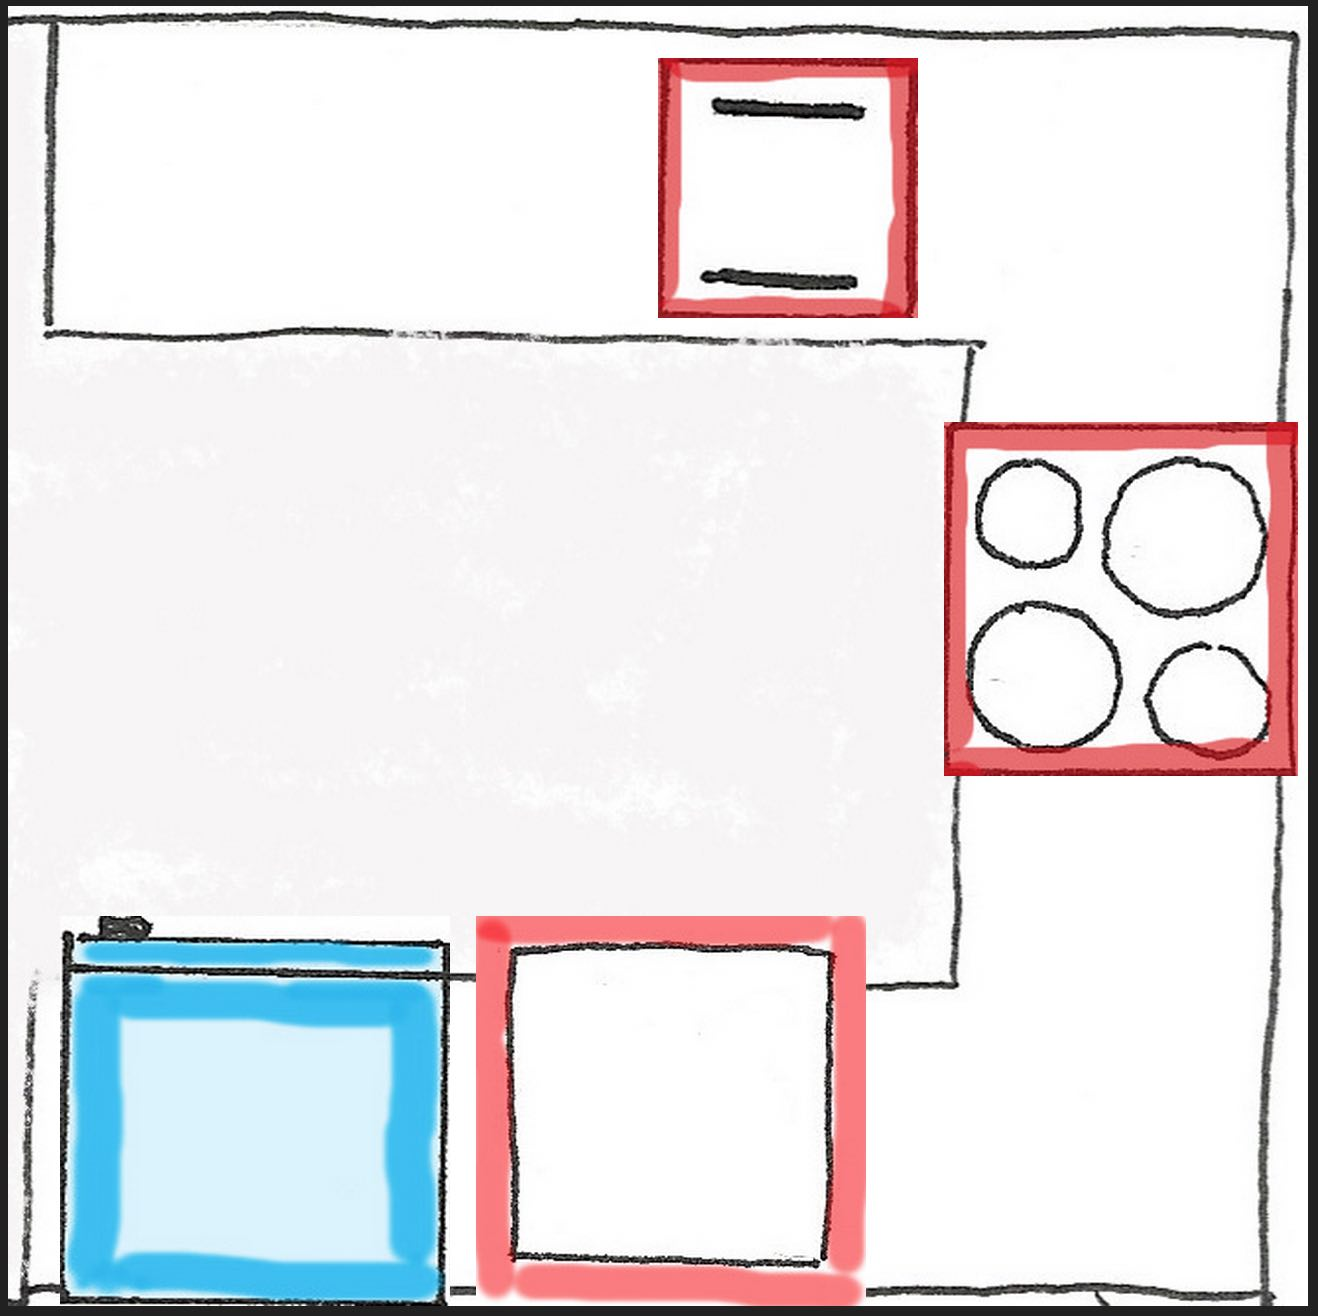
\includegraphics[scale=0.1]{fig/kitchen}
\caption{}
\label{fig:kitchenon}
\end{subfigure}
\begin{subfigure}{0.32\textwidth}
\centering
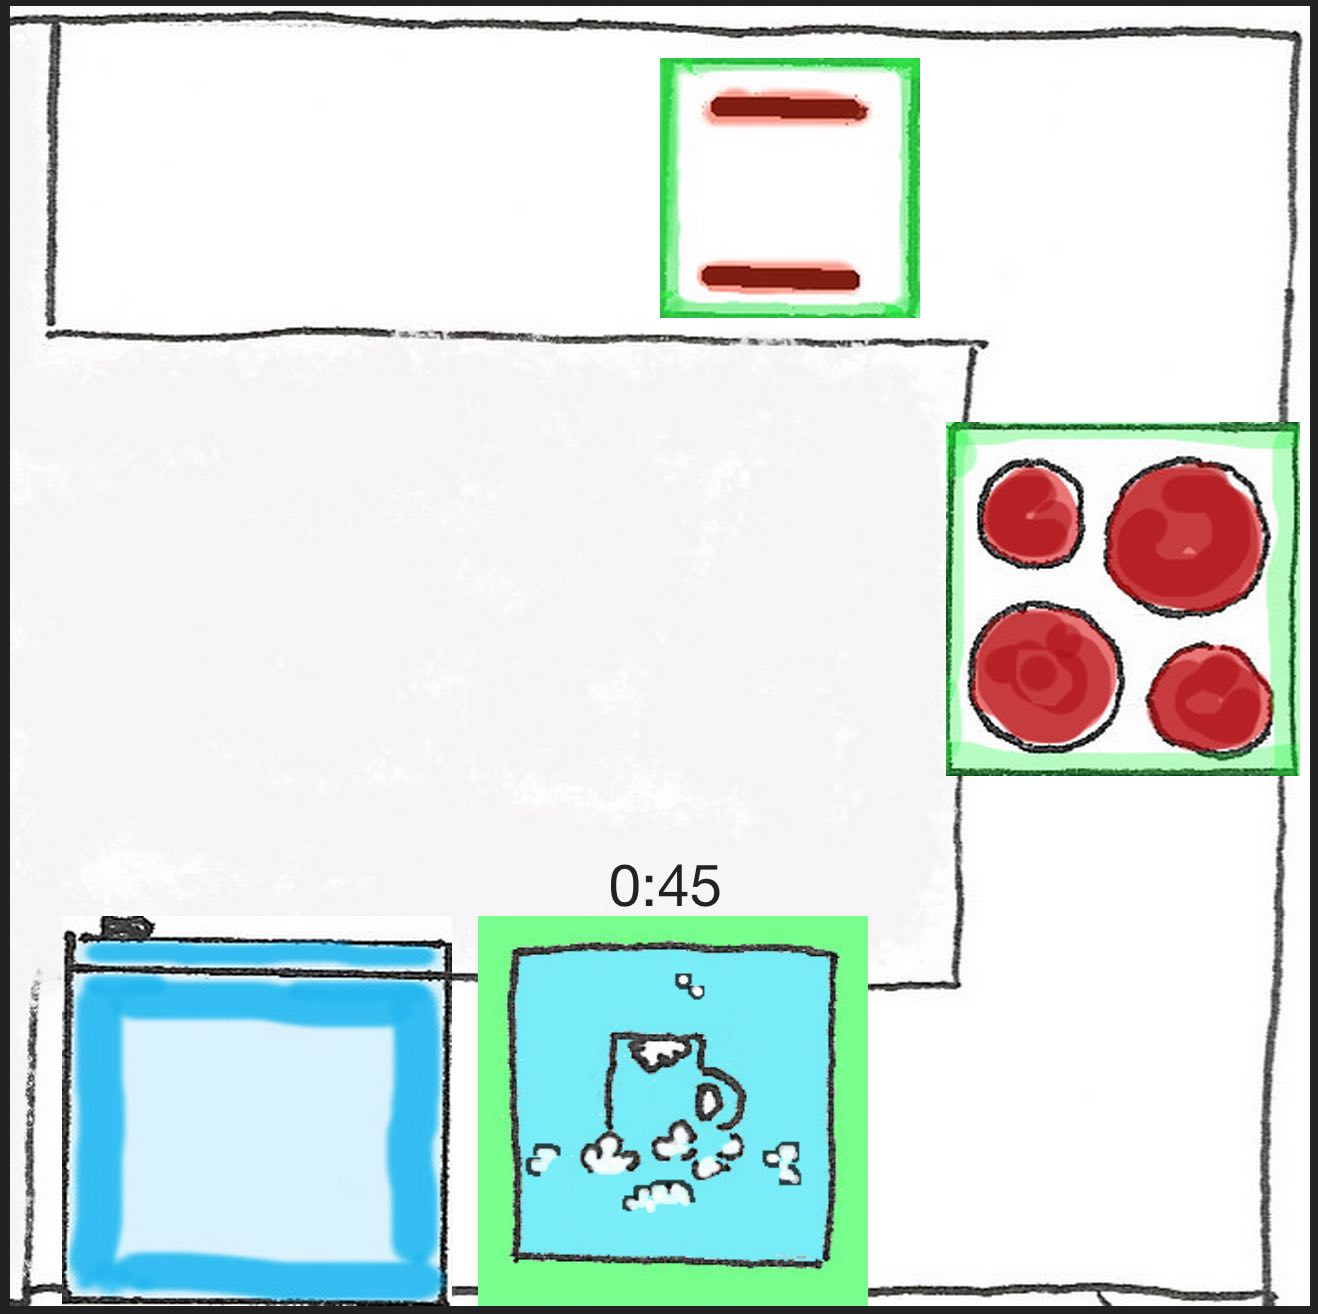
\includegraphics[scale=0.1]{fig/kitchen2}
\caption{}
\label{fig:kitchenoff}
\end{subfigure}
\caption{Apparater skrudd av og på}
\label{fig:kitchenonoff}
\end{figure}
\begin{figure}[ht]
\centering
\begin{subfigure}{0.32\textwidth}
\centering
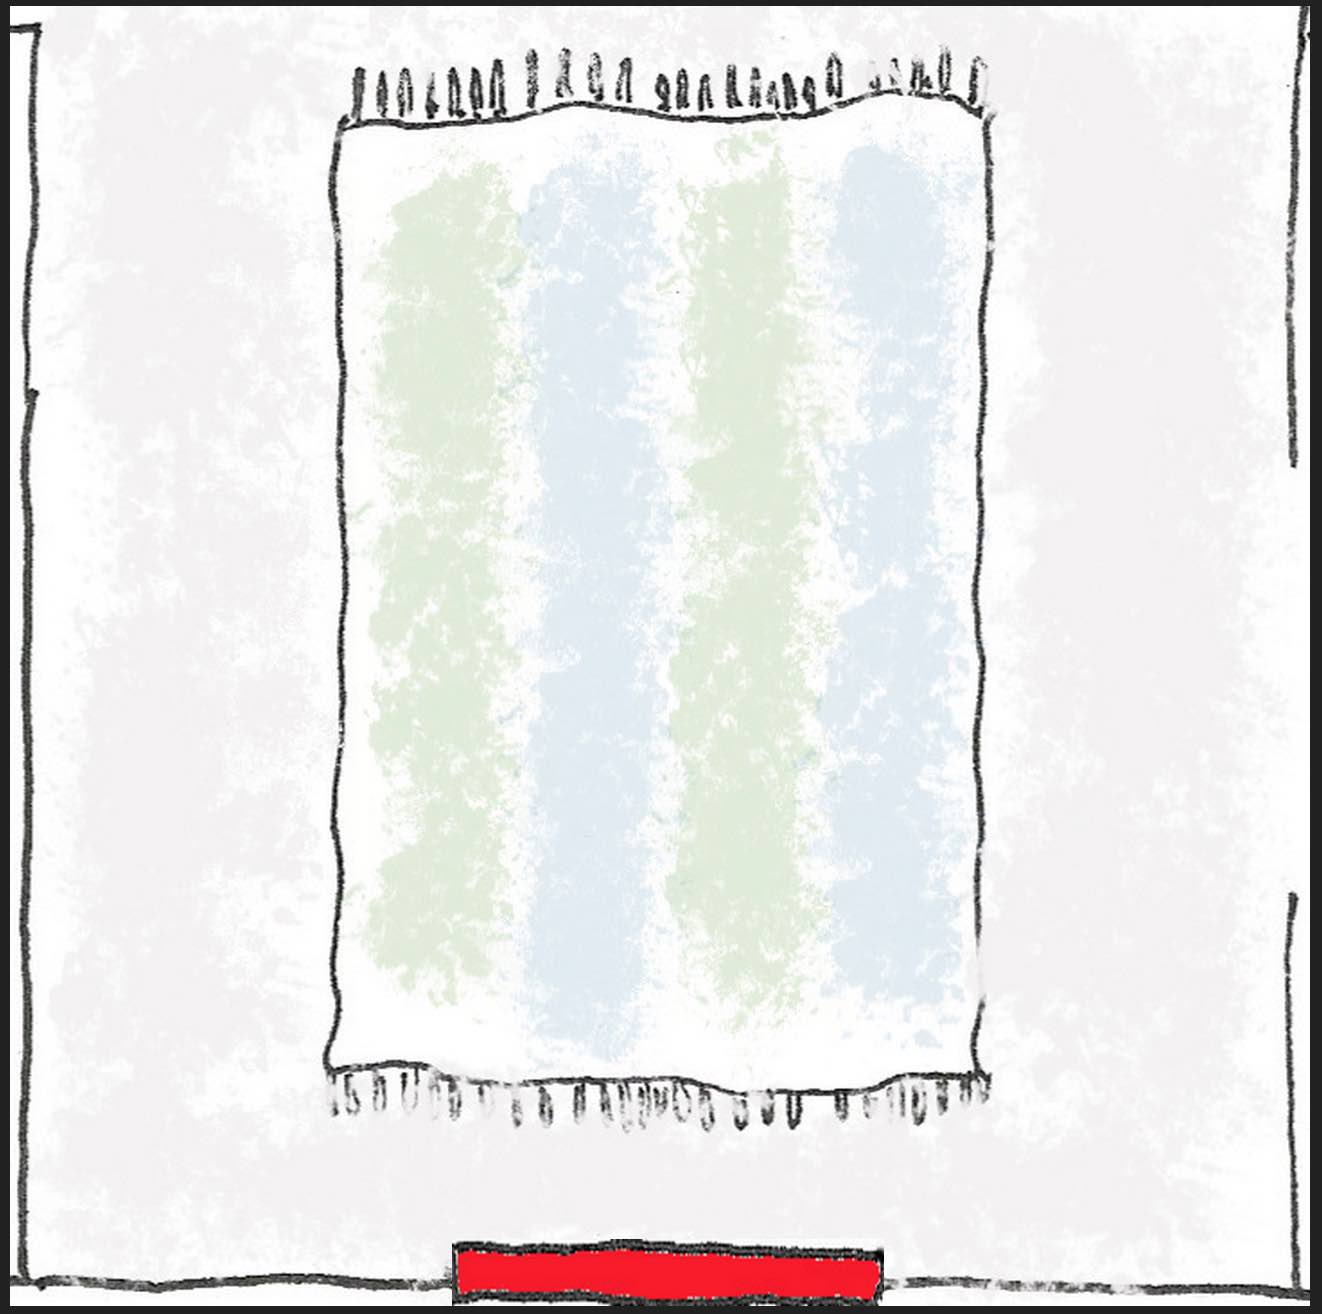
\includegraphics[scale=0.1]{fig/hall}
\caption{}
\label{fig:halllocked}
\end{subfigure}
\begin{subfigure}{0.32\textwidth}
\centering
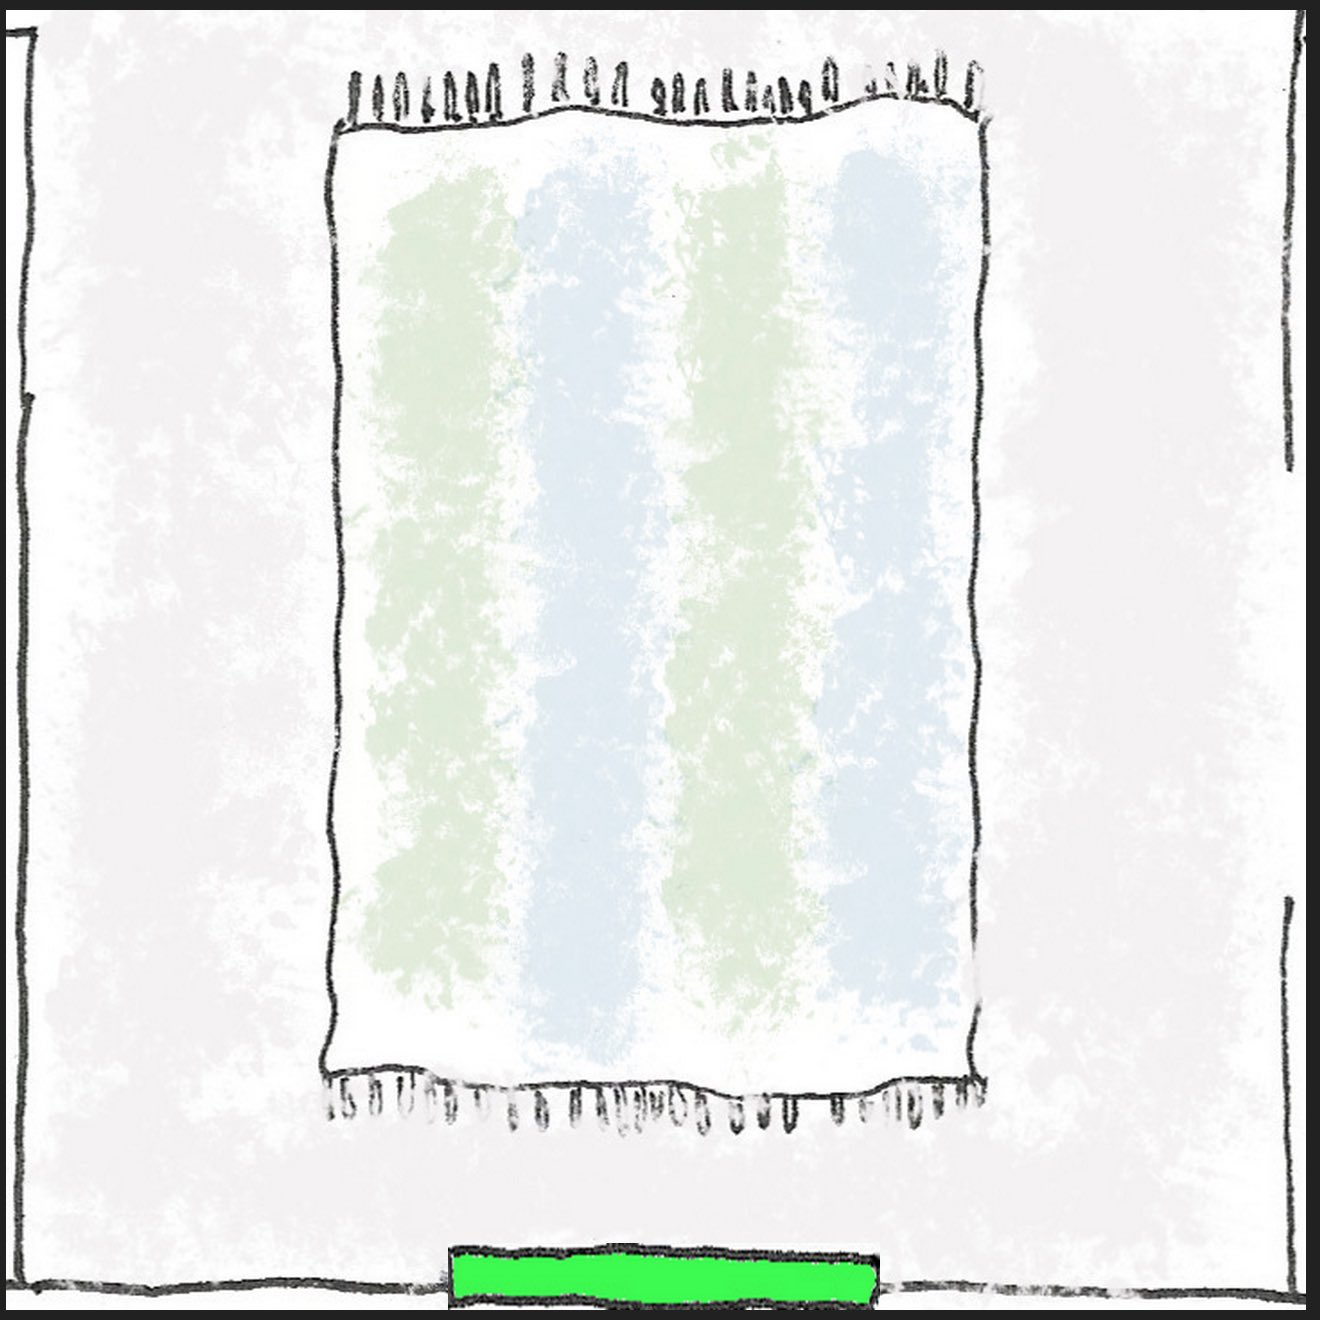
\includegraphics[scale=0.1]{fig/hall2}
\caption{}
\label{fig:hallopen}
\end{subfigure}
\caption{Gang med dør låst og ulåst}
\label{fig:halllockedopen}
\end{figure}
\begin{figure}[ht]
\centering
\begin{subfigure}{0.32\textwidth}
\centering
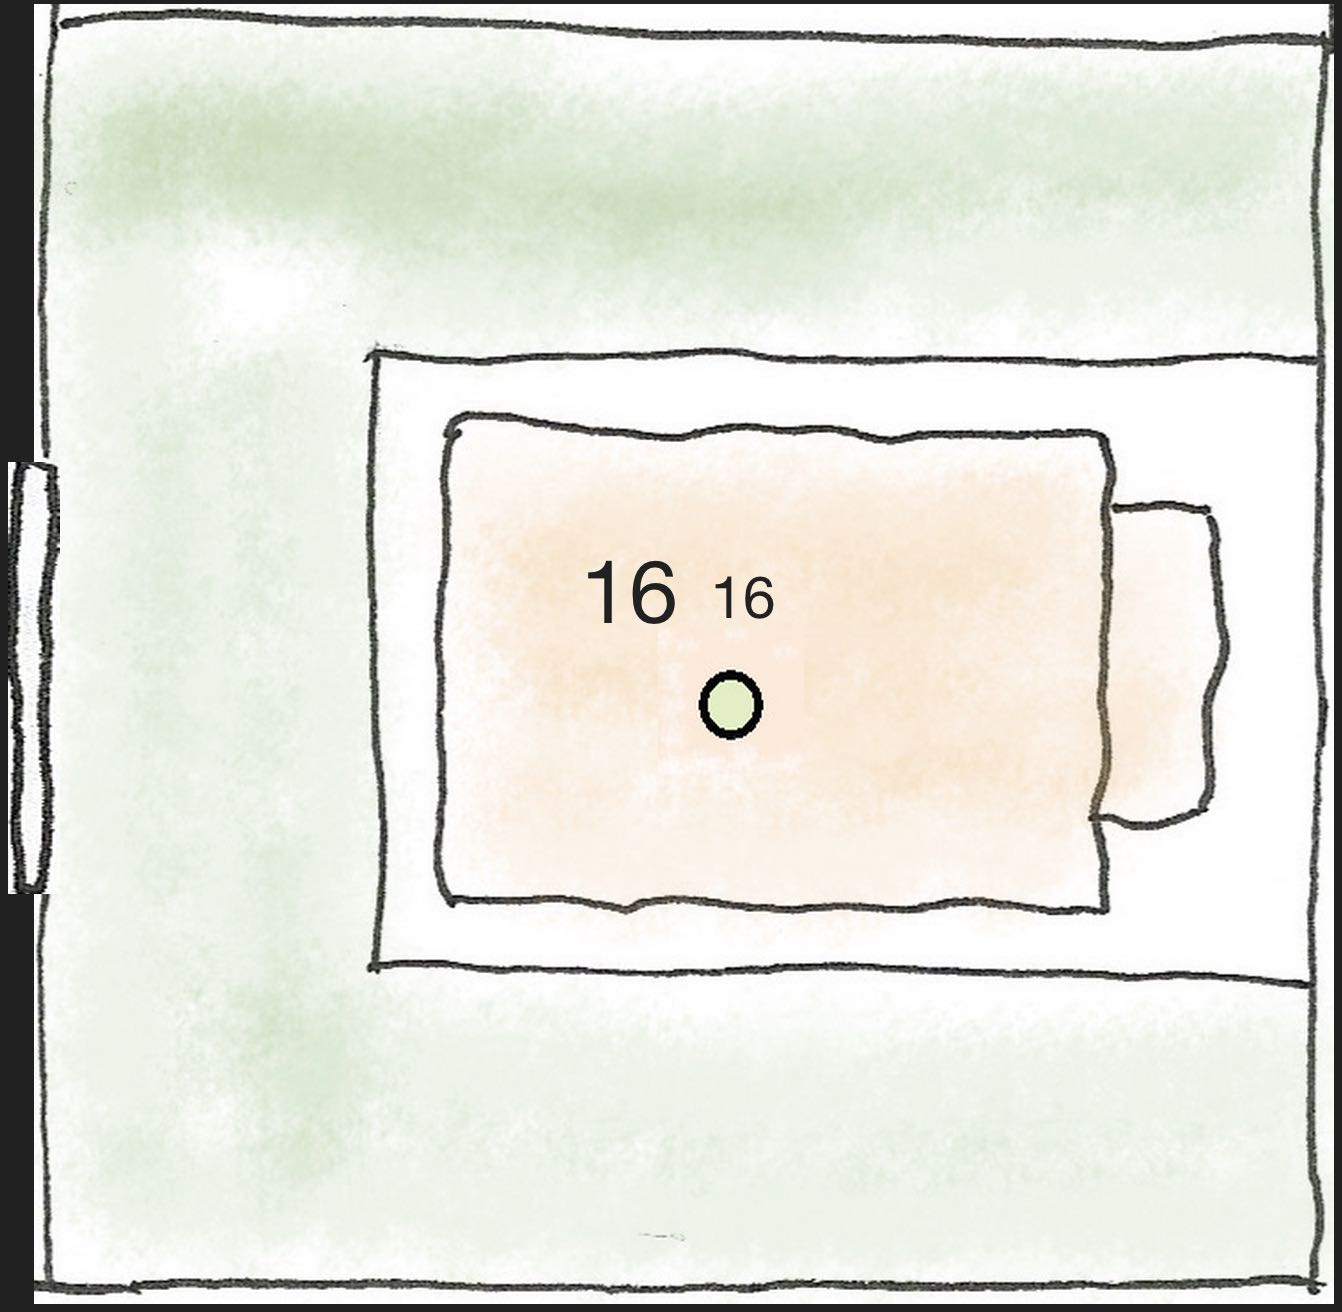
\includegraphics[scale=0.1]{fig/bedroom}
\caption{}
\label{fig:bedroomon}
\end{subfigure}
\begin{subfigure}{0.32\textwidth}
\centering
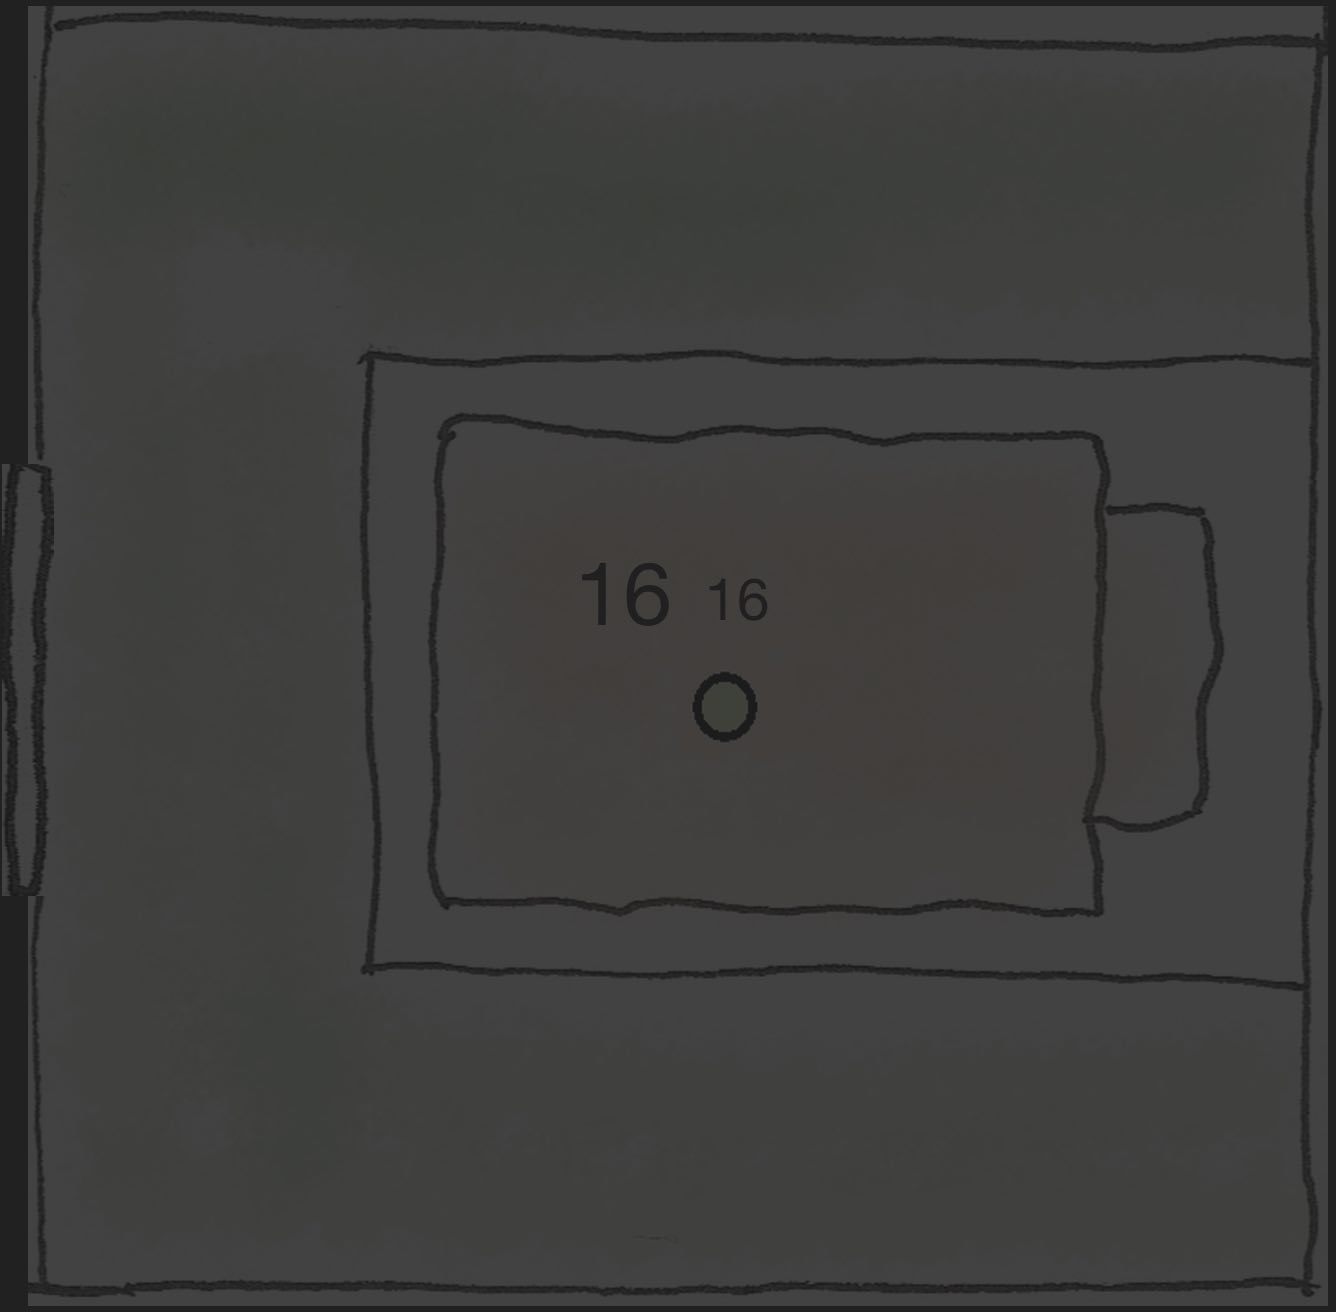
\includegraphics[scale=0.1]{fig/bedroom2}
\caption{}
\label{fig:bedroomoff}
\end{subfigure}
\caption{Soverom med lyset slått på og av}
\label{fig:bedroomonoff}
\end{figure}
Det er noen forsøk på å bruke farger symbolsk i grafikken. Elementer med klare rødfarger er avslått eller låst. Elementer med klare grønnfarger er på eller åpne. Figur \ref{fig:kitchenonoff} og \ref{fig:halllockedopen} viser forskjellene på elementer som er avslått/låst og som er på/åpne. Kjøleskapet er i en klar farge for å indikere at den kan interageres med. Ellers er elementene som utgjør bakgrunnen i grafikken i grå, utvaskede eller sjenerte farger. Noen av elementene i bakgrunnsgrafikken er også dynamiske og kan forandres av data om tilstanden til hjemmet. Dette gjelder dørene til bad og soverom, samt skittentøyskurven. Disse er dynamiske, men kan ikke interageres med. Dette bør gi mening ettersom det ikke er mulig å fjernstyre dørene i hjemmet. Det er også benyttet enkle animasjoner for å vise apparater som er aktive. Disse involverer forandring i lys fra tv, strømmende noter fra radio, og vaske- og oppvaskmaskiner med bevegelse og forandrene såpebobler. Figur \ref{fig:bedroomonoff} viser hvordan soverommet ser ut med lyset slått på/av. Lyset manipuleres ved å trykke på den runde, blekt gule sirkelen i midten av rommet.
\begin{figure}[ht]
\centering
\begin{subfigure}{0.32\textwidth}
\centering
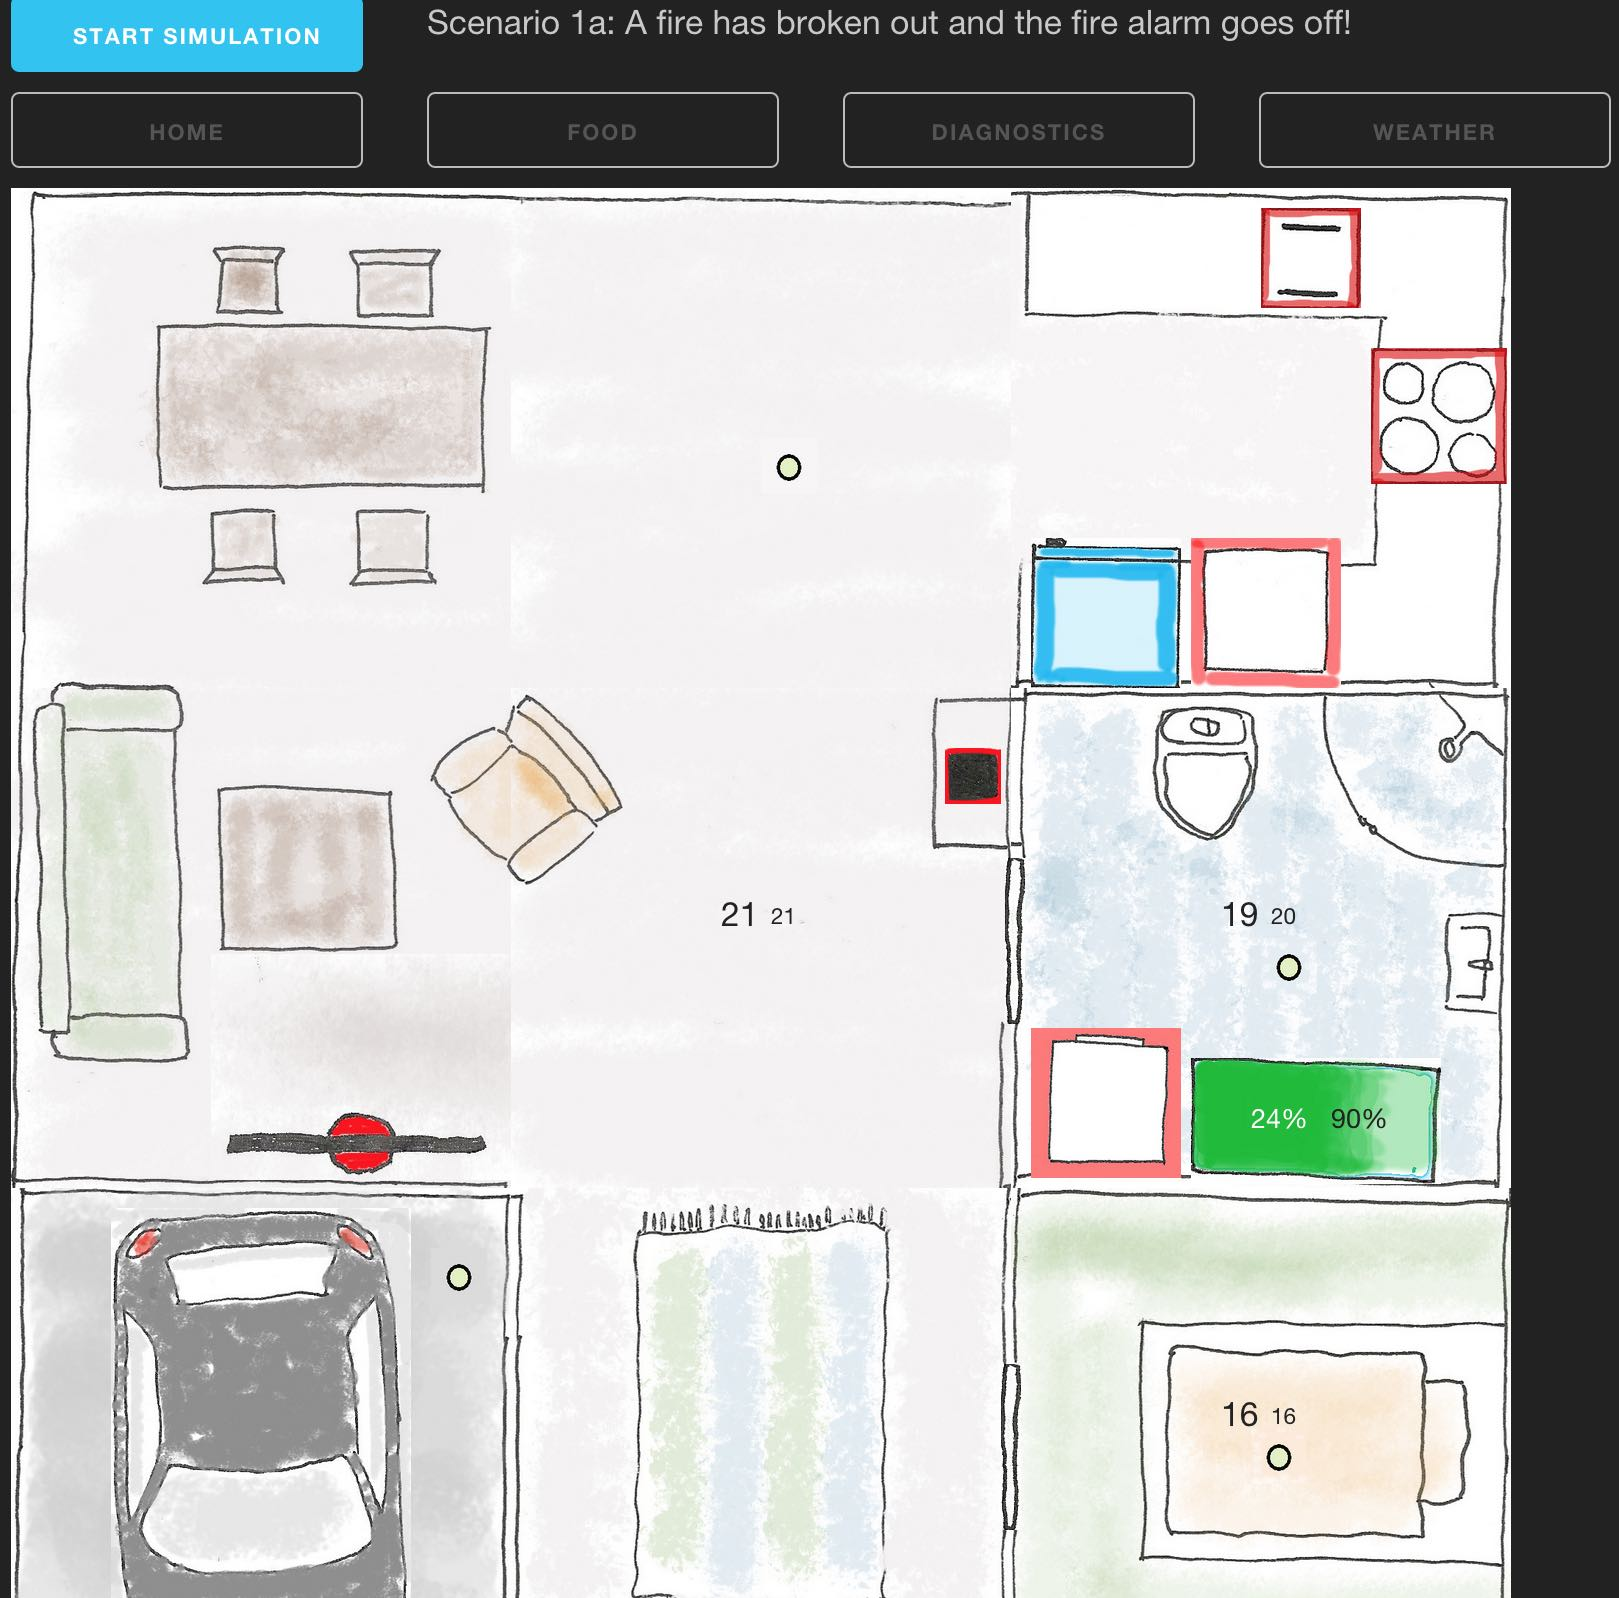
\includegraphics[width=5cm, height=5cm]{fig/scenario1a}
\caption{}
\label{fig:1a}
\end{subfigure}
\begin{subfigure}{0.32\textwidth}
\centering
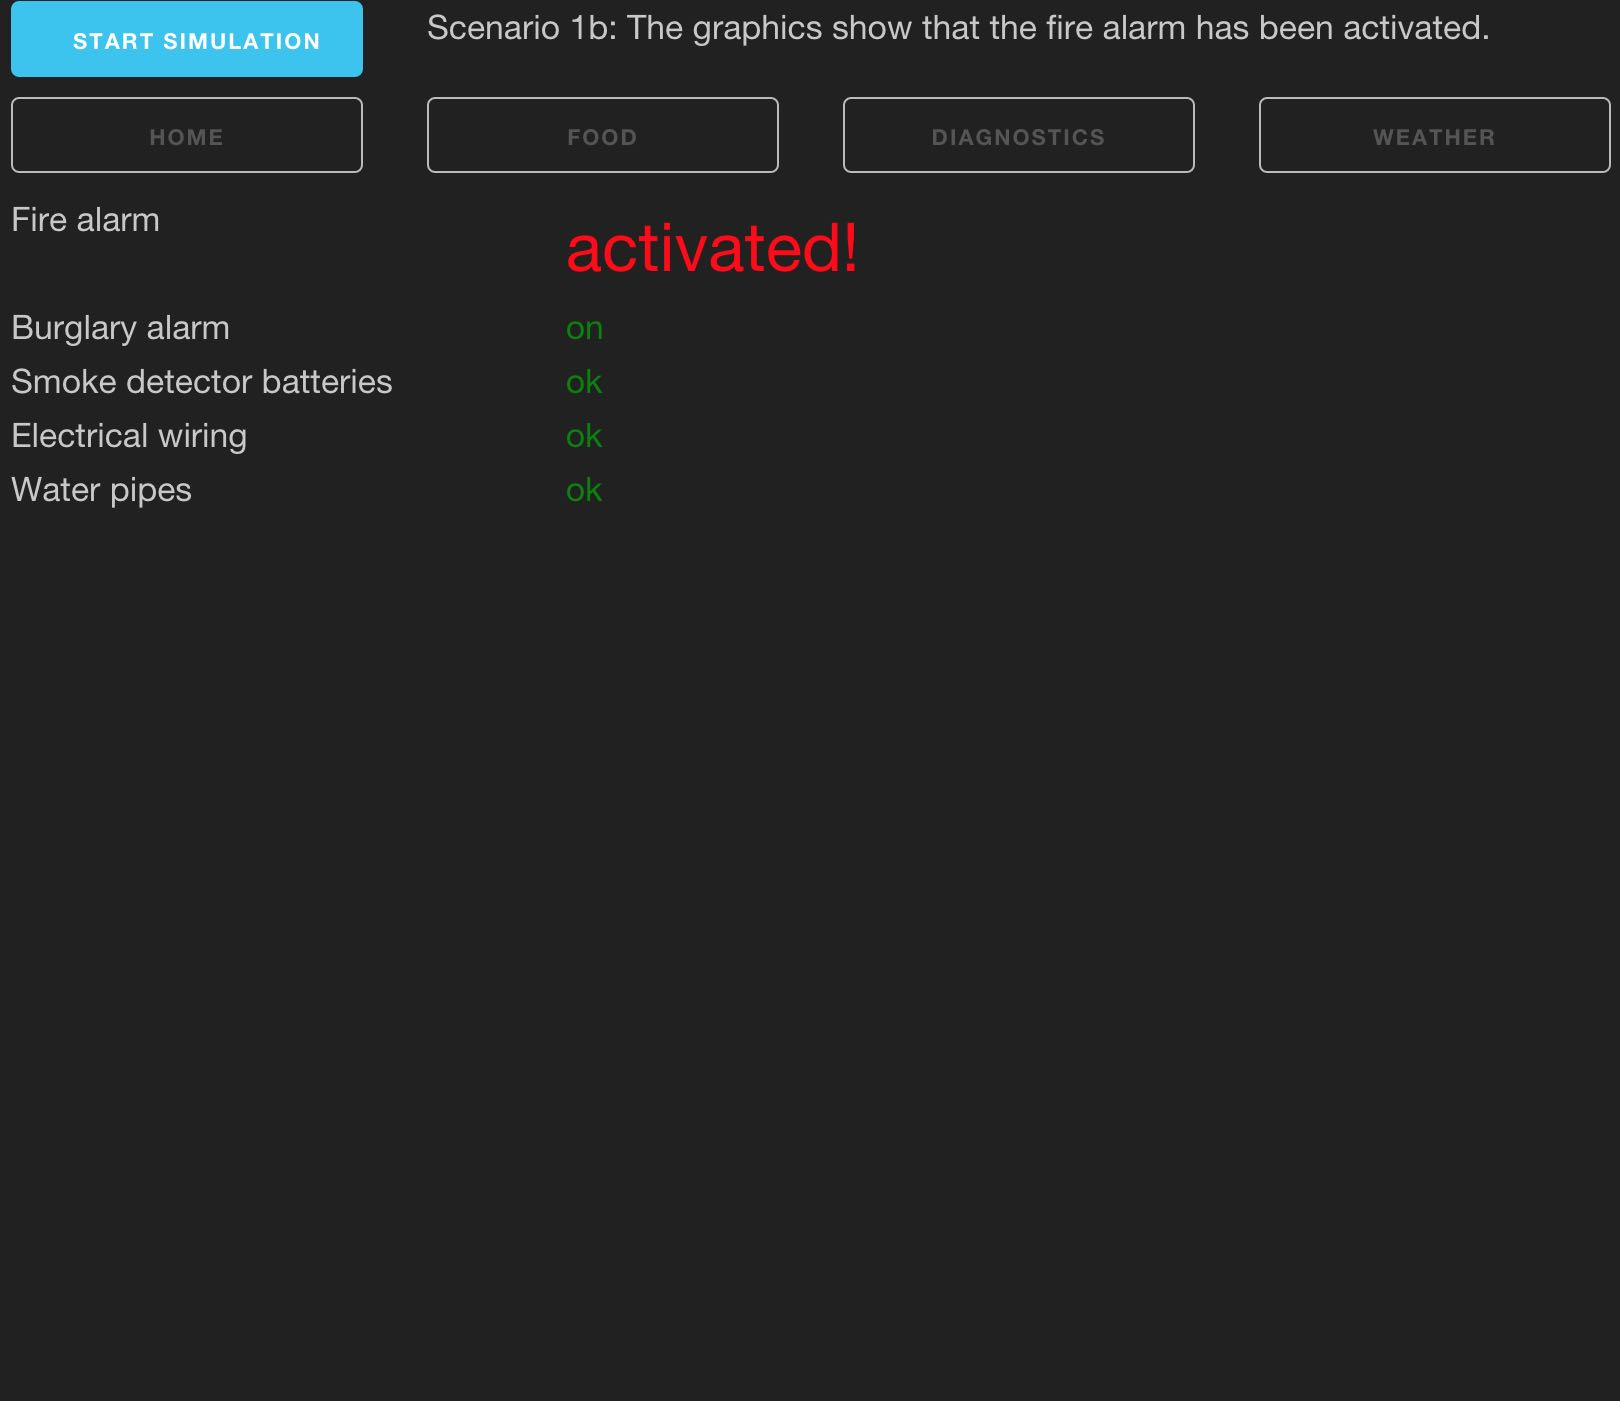
\includegraphics[width=5cm, height=5cm]{fig/scenario1b}
\caption{}
\label{fig:1b}
\end{subfigure}
\caption{Scenario 1}
\label{fig:scenario1}
\end{figure}
Dersom systemet kan forstå konteksten i hjemmet kan irrelevant data fjernes og grafikk som er generes etter behov i øyeblikket. Tradisjonelt er konteksten definert av brukerinteraksjon. Søkeord og valg i menyer gir programvaren informasjon om hva som er viktig og gir den muligheten til å presentere relevante resultater. Kontekstinformasjon kan komme fra sensorinformasjon fra det fysiske miljøet, historie over tidligere valg og gjennom interaksjon med brukeren. Det smarte hjemmet vil være fylt til randen av sensorer og informasjon fra det fysiske miljøet, så dette kan regnes som den viktigste kontekstinformasjonen. Annen informasjon, som tid og hjemmets posisjon, gjør det enkelt å hente informasjon fra eksterne kilder, som å spørre \emph{API}-er etter værutsiktene eller brukerens kalenderinformasjon.
\begin{figure}[ht]
\centering
\begin{subfigure}{0.23\textwidth}
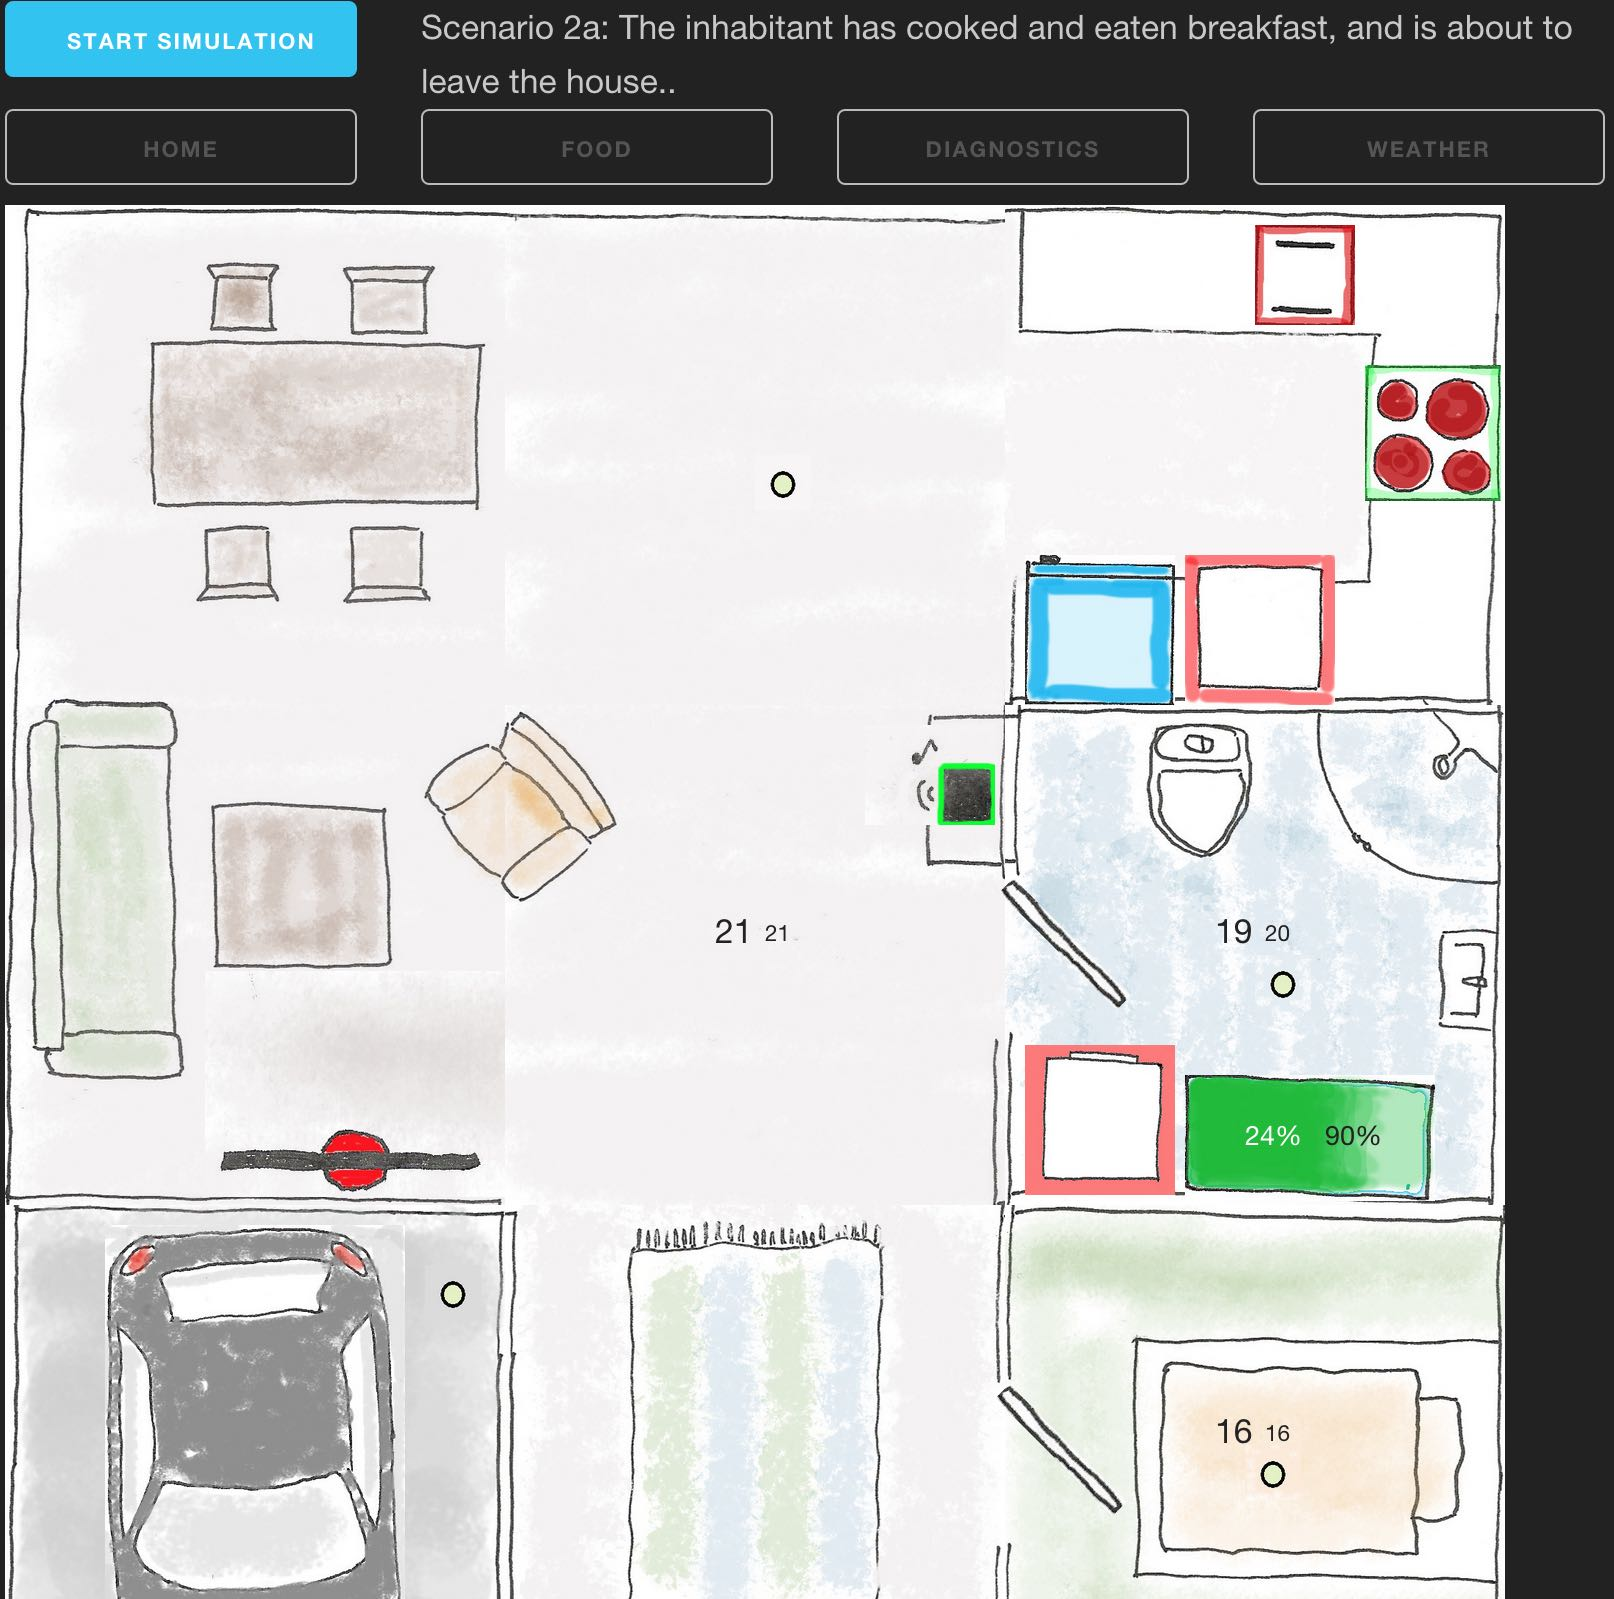
\includegraphics[width=4cm, height=4cm]{fig/scenario2a}
\caption{}
\label{fig:2a}
\end{subfigure}
\begin{subfigure}{0.23\textwidth}
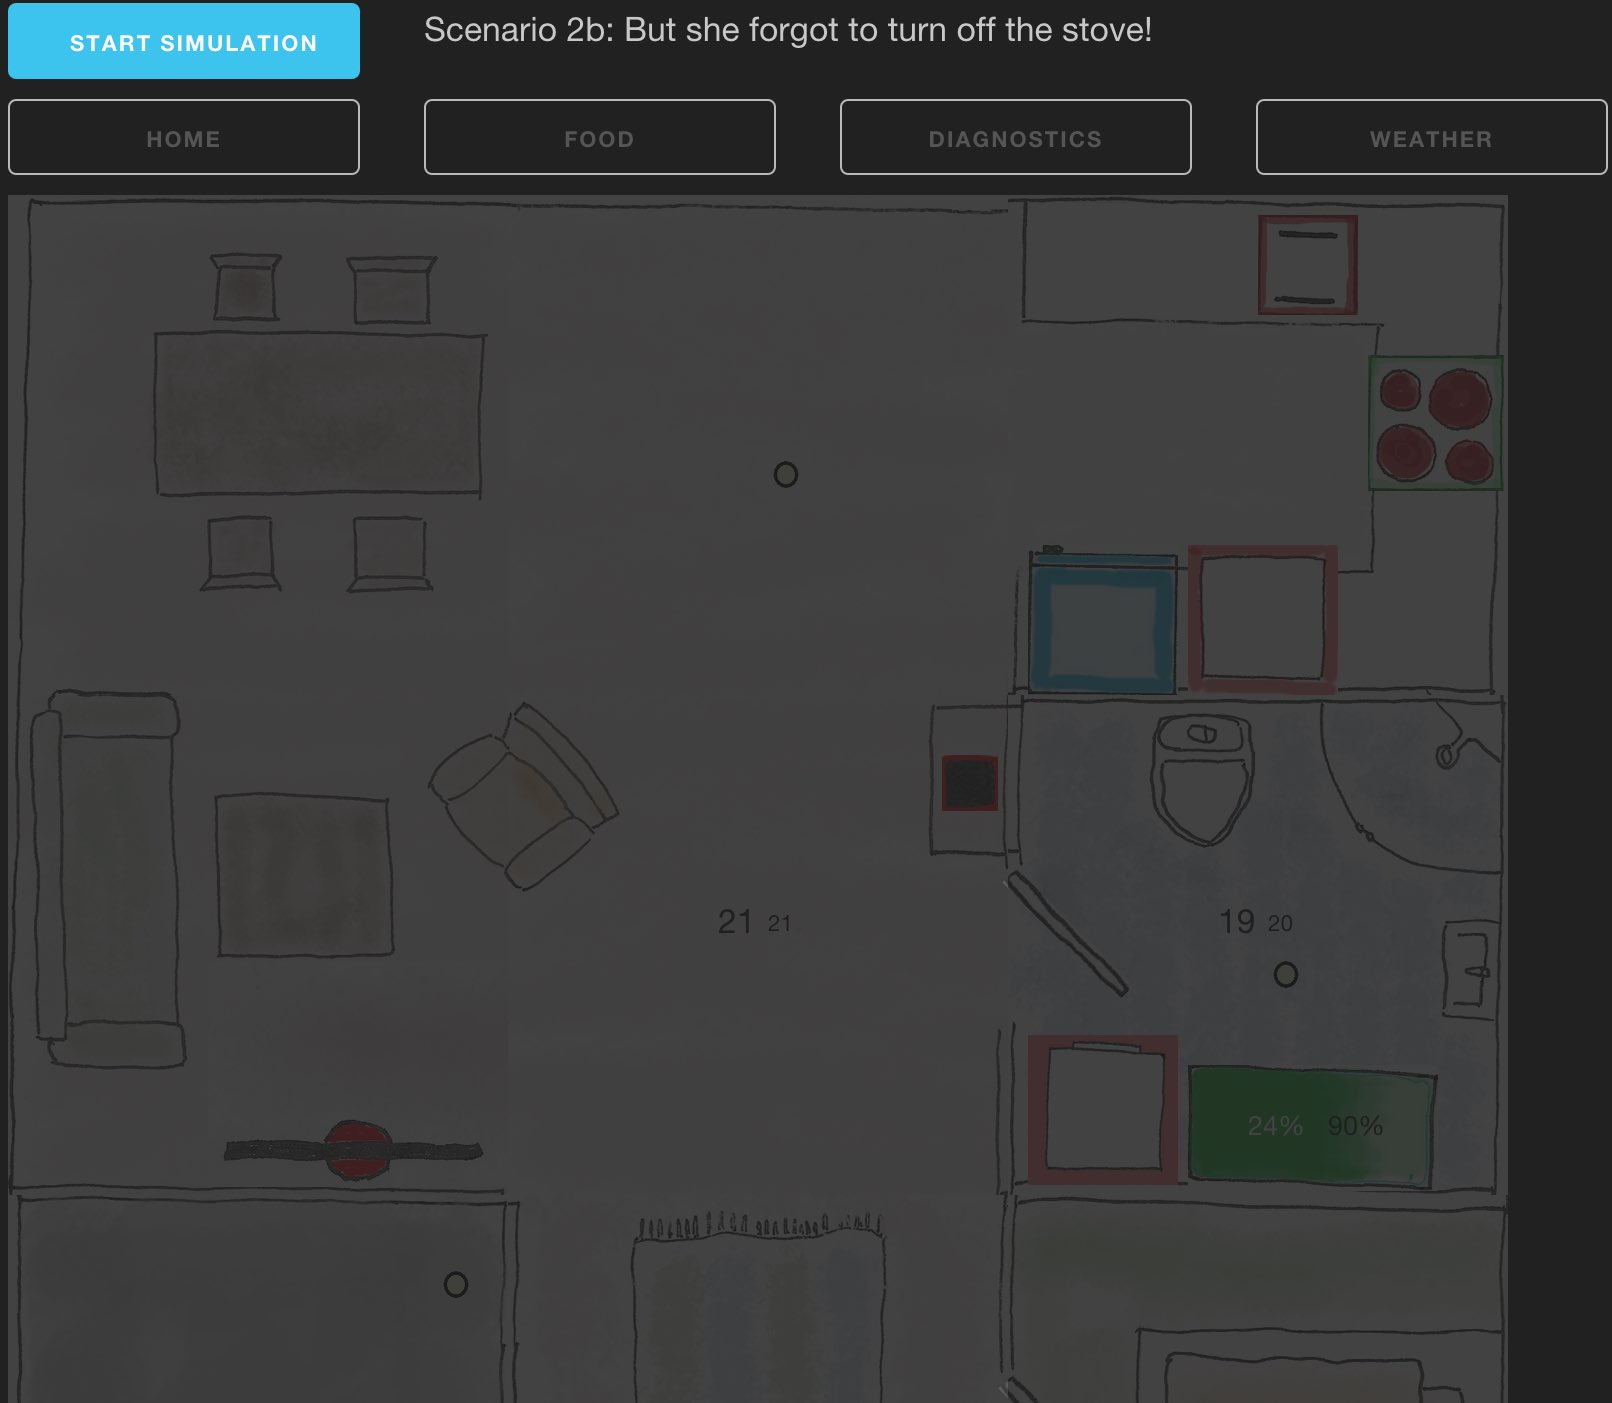
\includegraphics[width=4cm, height=4cm]{fig/scenario2b}
\caption{}
\label{fig:2b}
\end{subfigure}
\begin{subfigure}{0.23\textwidth}
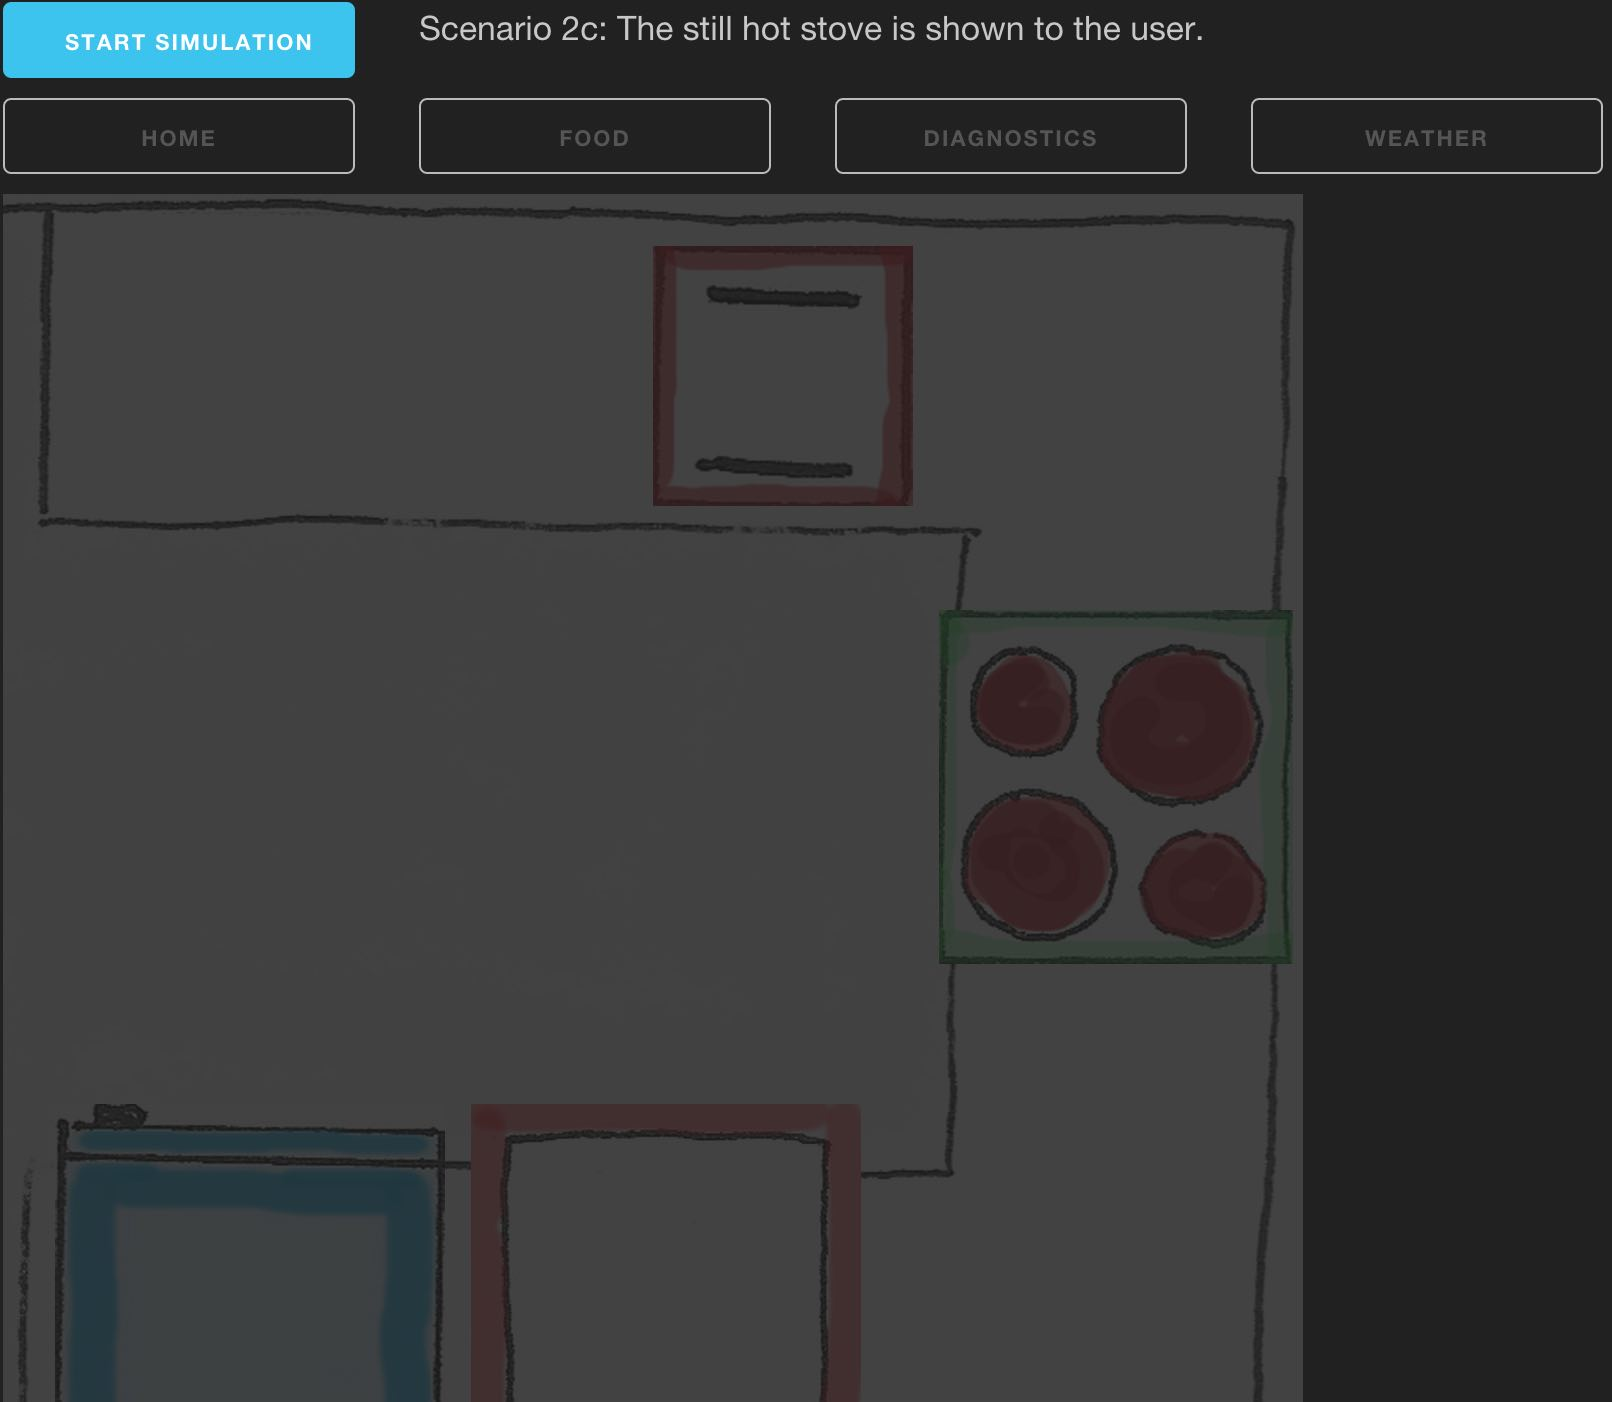
\includegraphics[width=4cm, height=4cm]{fig/scenario2c}
\caption{}
\label{fig:2c}
\end{subfigure}
\caption{Scenario 2}
\label{fig:scenario2}
\end{figure}
Systemet kan også bruke historie til å forstå kontekst. Den nåværende konteksten, eller i det minste en god tilnærming, kan bli gjettet basert på en historie av tidligere miljøer og interaksjoner. Å gjette basert på den siste kjente verdien, er den enkleste formen for gjetning. Systemet gjetter den nåværende konteksten til å være den samme som den forrige. Dette er rimelig i mange situasjoner der konteksten forandrer seg lite over et kort tidsrom. For eksempel, hvis brukeren i går foretrakk å se på en grafisk representasjon av hele huset, er den samme brukeren sannsynligvis interessert i å se det samme den neste dagen. Det ville ikke vært rimelig å neste dag starte med å vise informasjon om energiforbruket i huset. Hvis lite, eller ingenting er forandrert bør programvaren vise den samme informasjonen som var foretrukket sist.
\begin{figure}[ht]
\centering
\begin{subfigure}{0.32\textwidth}
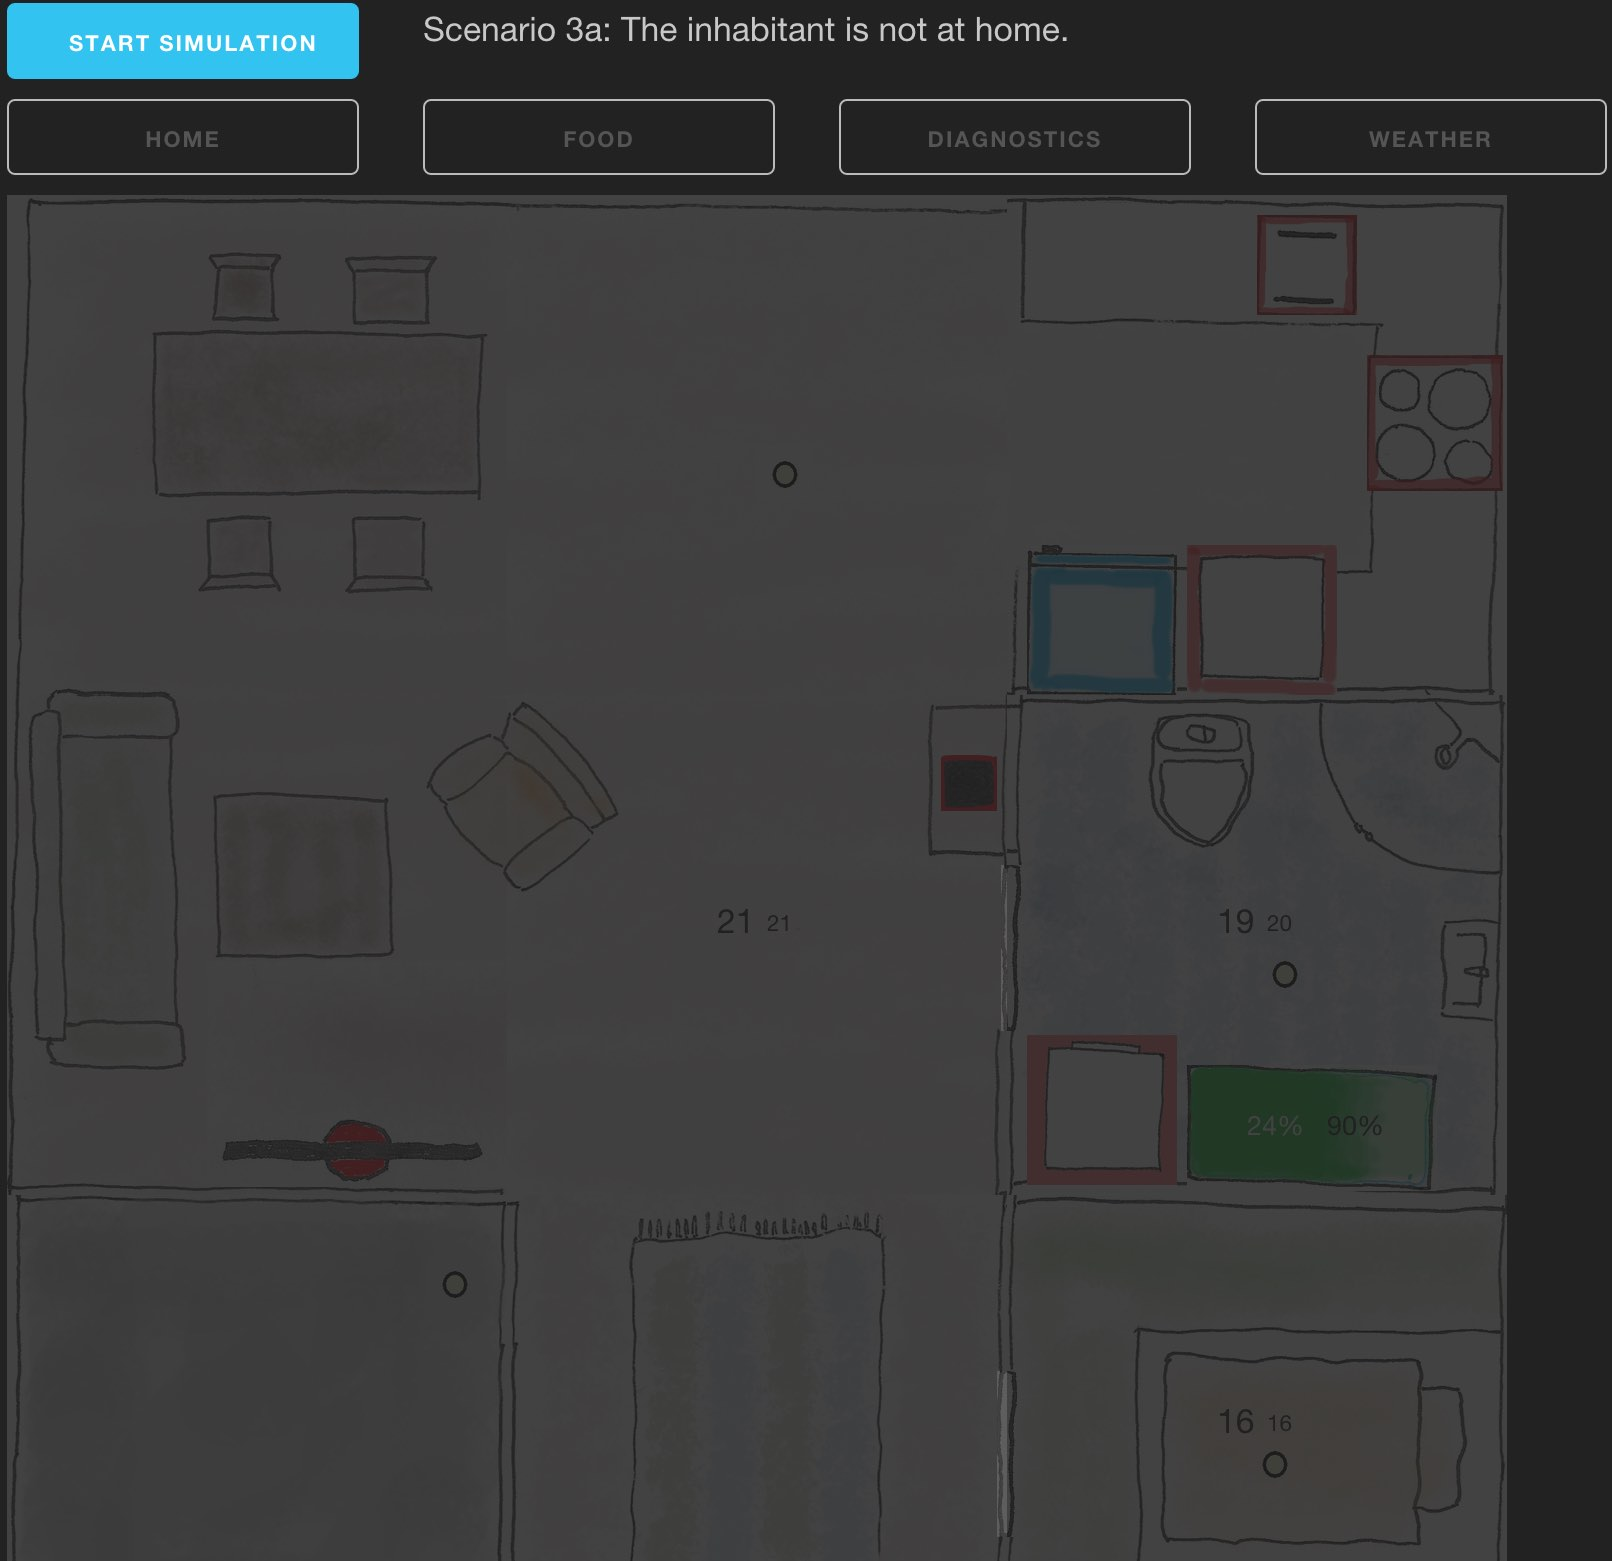
\includegraphics[width=5cm, height=5cm]{fig/scenario3a}
\caption{}
\label{fig:3a}
\end{subfigure}
\begin{subfigure}{0.32\textwidth}
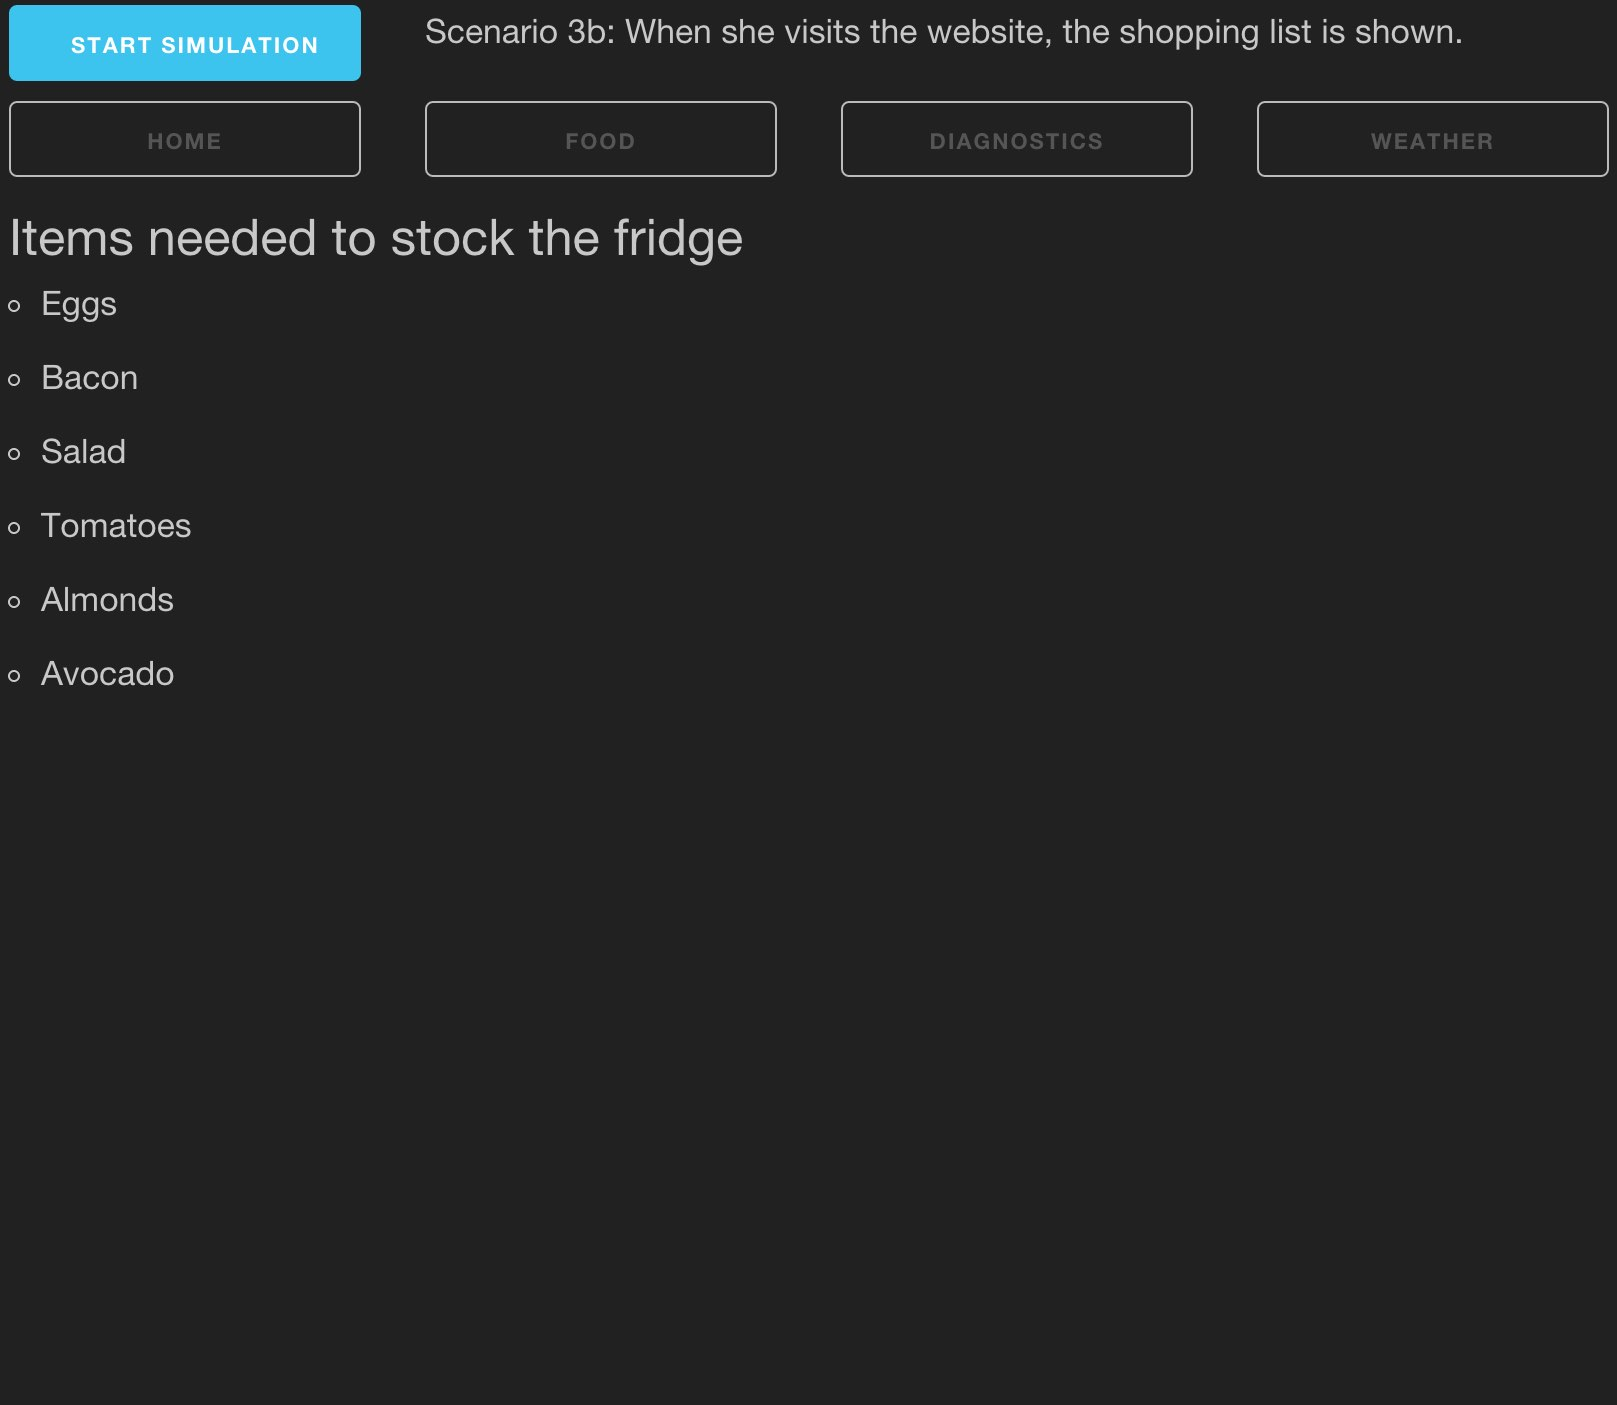
\includegraphics[width=5cm, height=5cm]{fig/scenario3b}
\caption{}
\label{fig:3b}
\end{subfigure}
\caption{Scenario 3}
\label{fig:scenario3}
\end{figure}
\begin{figure}[ht]
\centering
\begin{subfigure}{0.32\textwidth}
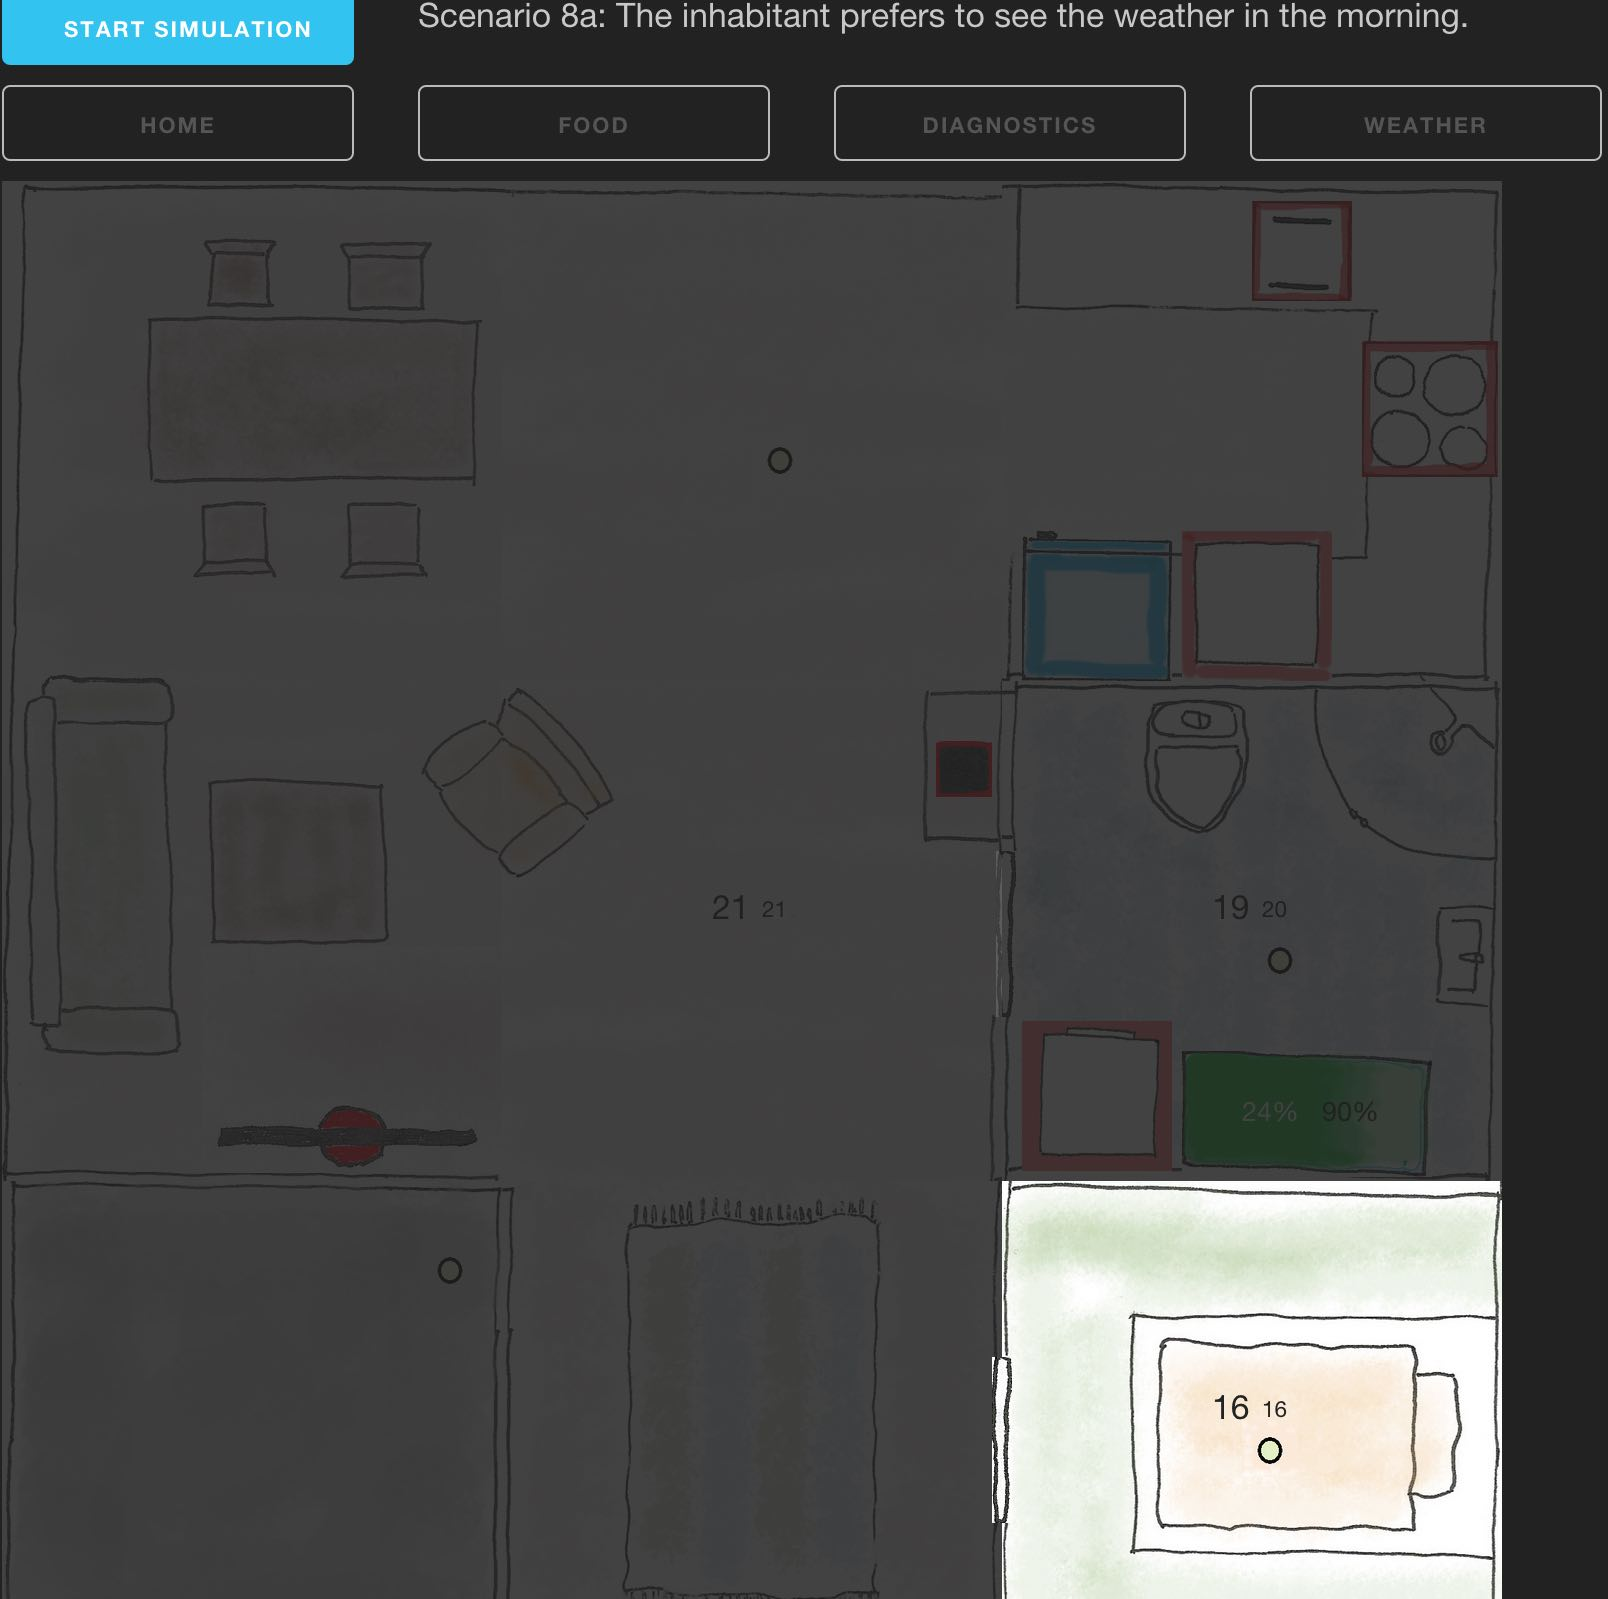
\includegraphics[width=5cm, height=5cm]{fig/scenario8a}
\caption{}
\label{fig:8a}
\end{subfigure}
\begin{subfigure}{0.32\textwidth}
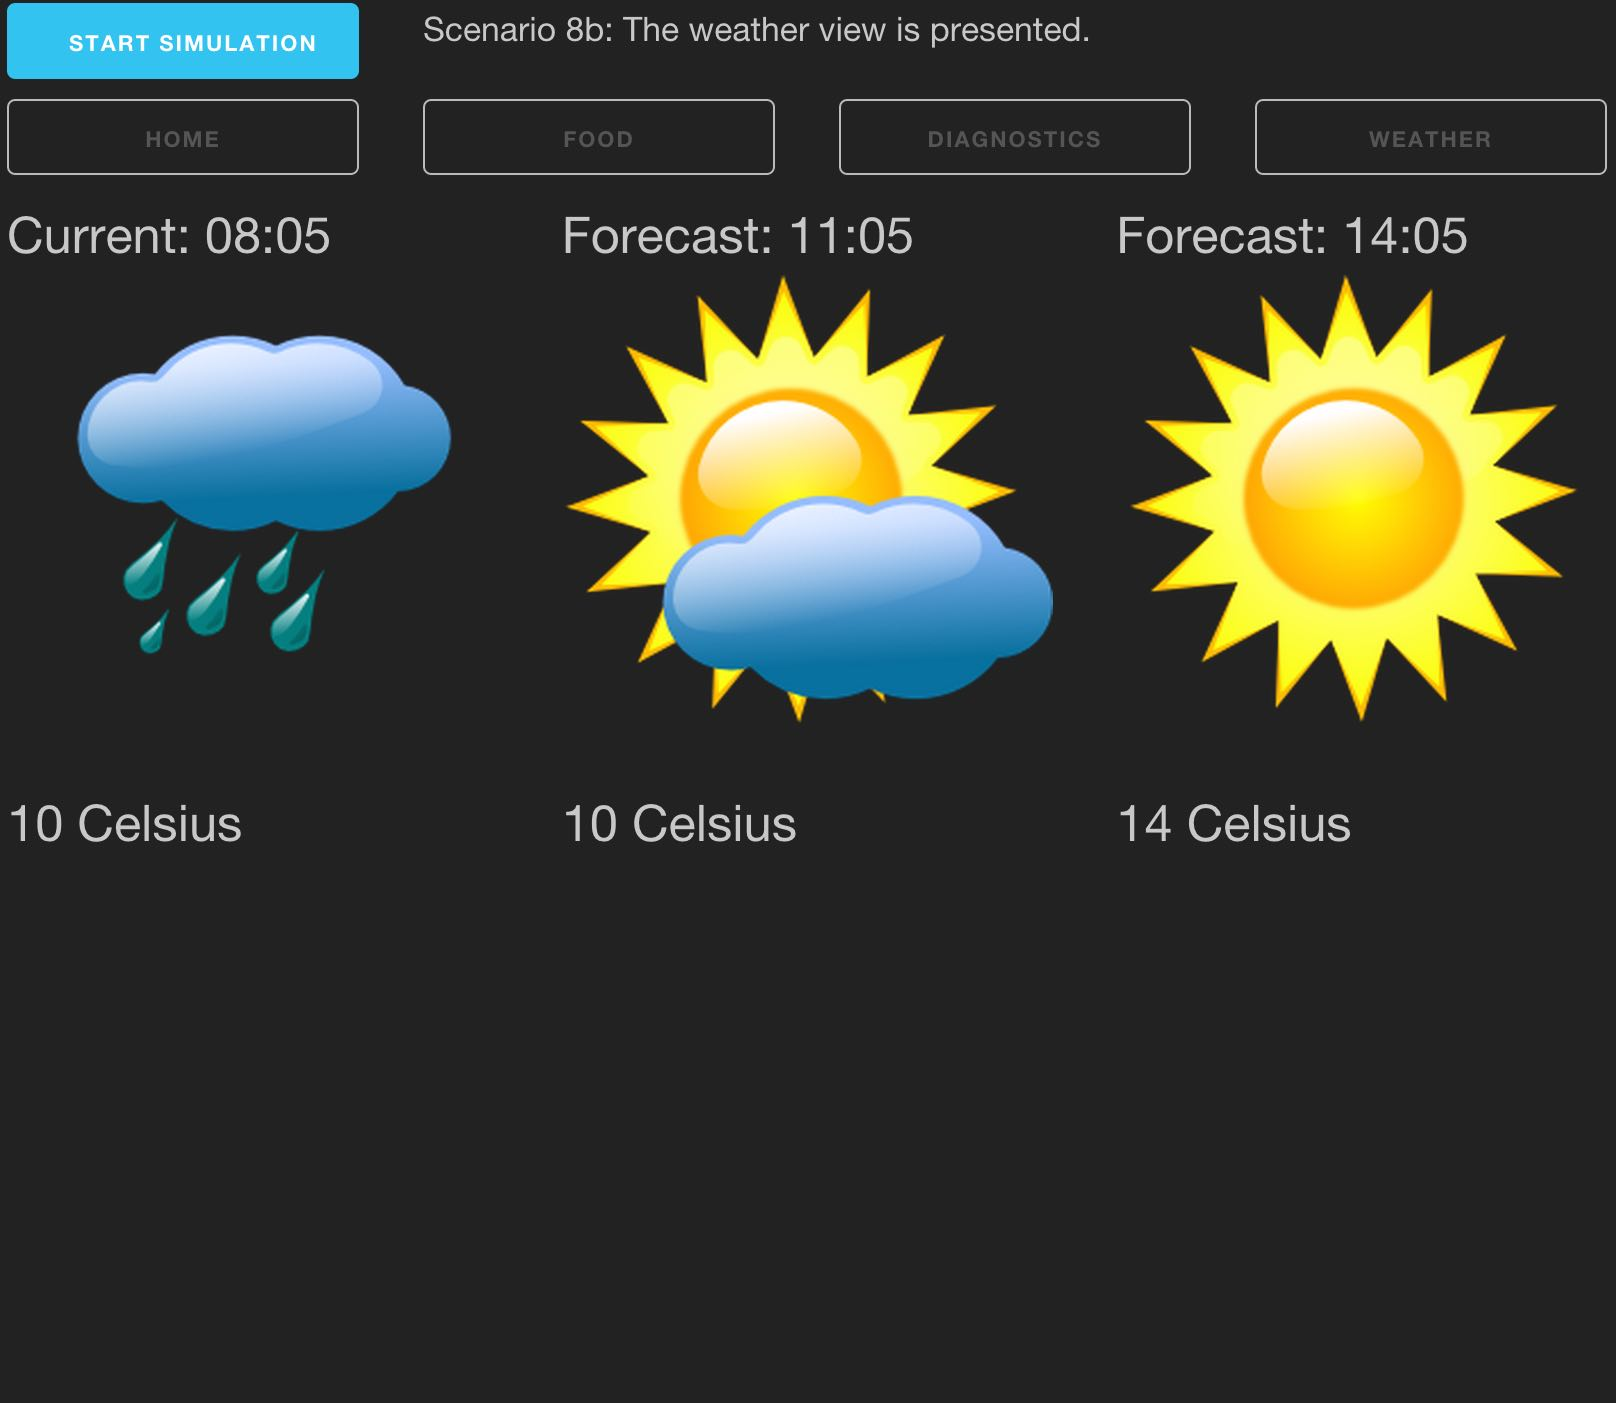
\includegraphics[width=5cm, height=5cm]{fig/scenario8b}
\caption{}
\label{fig:8b}
\end{subfigure}
\caption{Scenario 8}
\label{fig:scenario8}
\end{figure}
Dersom systemet kan forstå så mye som mulig fra miljøet og fra historie bør den i det minste klare å produsere et rimelig utgangspunkt for å gi brukeren det hun er interessert i. Mesteparten av brukerens interaksjon blir derfra å korrigere eller bekrefte programmets gjetninger.

For å demonstrere hvordan grafikken forandrer seg dynamisk basert på dataene fra hjemmet implementerte jeg en simulering som går gjennom et utvalg scenarier. Disse scenariene er definert av regler. Reglene sier hva som skal vises dersom visse data forekommer. Figur \ref{fig:scenario1} viser hva som skjer dersom brannalarmen aktiveres. Dersom brukeren besøker nettstedet blir hun straks møtt med tydelig informasjon om at brannalarmen har blitt aktivert. Figur \ref{fig:scenario2} viser hvordan hjemmet presenteres dersom brukeren forlater hjemmet uten å skru av stekeplata. Den potensielt farlige situasjonen settes i fokus og lar brukeren enkelt skru av plata dersom det er ønskelig. I figur \ref{fig:scenario3} er hjemmet i en nøytral tilstand og brukeren er ikke i hjemmet. Han har laget en regel som sier at kjøleskapets handleliste skal vises i denne situasjonen. Dette er den informasjonen om hjemmet denne brukeren som oftest er interessert i når han er ute og går. Til sist, i figur \ref{fig:scenario8} viser systemet været om morgenen.\\

\subsection{Resultater}
\subsubsection*{Gestegjenkjennelse gjennom fotodioder}
Resultatet av dette eksperimentet vises i følgende tabell. Tabellen viser graden av suksess de lineære klassifiseringsalgoritmene oppnådde.
\begin{table}[h!]
\centering
\begin{tabular}{|| c c c c c ||}
\hline
\% korrekt klassifisering & Algoritme & Antall gester & Treningseksempler/gest \\ [0.5ex] 
 \hline\hline
 96.22 +- 0.34 & SVM v/libsvm & 10 & 50 \\ 
 \hline
 96.02 +- 0.35 & SVM v/liblinear & 10 & 50 \\
 \hline
 94.58 +- 0.34 & Logistisk regresjon & 10 & 50 \\
 \hline
\end{tabular}
\caption{Klassifisering av 10 gester}
\label{table:results}
\end{table}
Modellene er trent og testet 100 ganger med tilfeldige utgangspunkt og resultatene er oppgitt med 95\% konfidensintervall.\\

\subsubsection*{Multimodal interaksjon gjennom tale og gester}
Dette eksperimentets resultat ble en argumentasjon for begrenset tale i hjemmet. Det ble også foreslått en måte å håndtere multimodaliteten på, med tråder, en felles kø og \emph{late fusion}.

\subsubsection*{Kombinasjoner}
\begin{table}[h!]
\centering
\begin{tabular}{|| c c c c ||}
\hline
\% korrekt klassifisering & Algoritme & Antall gester & Treningseksempler/gest \\ [0.5ex] 
 \hline\hline
 94,04 +- 0.68 & SVM m/liblinear & 10 & 10 \\
 \hline
 93,24 +- 0.75 & Logistisk regresjon & 10 & 10 \\
 \hline
 92,52 +- 0.75 & SVM m/libsvm & 10 & 10 \\ 
 \hline
\end{tabular}
\caption{Klassifisering av de samme 10 gestene fra eksperiment 1}
\label{table:results-foursensors}
\end{table}
Modellene er trent og testet 100 ganger med tilfeldige utgangspunkt.
\begin{table}[h!]
\centering
\begin{tabular}{|| c c c c ||}
\hline
\% Korrekt klassifisering & Algoritme & Antall gester & Treningseksempler/gest\\ [0.5ex] 
 \hline\hline
 93,68 +- 0.55 & SVM m/libsvm & 42 & 10 \\ 
 \hline
 92,74 +- 0.49 & Logistisk regresjon & 42 & 10 \\
 \hline
 92,54 +- 0.52 & SVM m/liblinear & 42 & 10 \\[1ex]
 \hline
\end{tabular}
\caption{Klassifisering av 42 gester}
\label{table:results-foursensors-42}
\end{table}
Med kun 10 treningseksempler av hver av de 42 gestene oppnås en suksessrate på 93.68\%. Modellene er trent og testet 100 ganger med tilfeldige utgangspunkt. Resultatene er oppgitt med 95\% konfidensintervall.

Eksperimentet har i tillegg vist hvordan dimming kan implementeres med en nærhetssensor.

\subsubsection*{Kontekstdrevet brukergrensesnitt}
Dette eksperimentet resulterte i en implementasjon av et grafisk brukergrensesnitt, designet delvis etter prinsipper fra grafisk design. Utviklingen ble en utforskning av et dynamiske brukergrensesnitt, drevet av kontekstdata fra hjemmet, framfor interaksjon med brukeren. Eksperimentet benyttet prioriterte regler for å avgjøre hvordan dataene burde presenteres.